%% Copyright (C) 2018 Adrien Blanchet
%%

%%%%%%%%%%%%%%%%%%%%%%%%%%%%%%%%%%%%%%%%
%             Chapitre Results               %
%%%%%%%%%%%%%%%%%%%%%%%%%%%%%%%%%%%%%%%%

\chapter{Résultats et discutions}
\label{chap:chapitre_results}

\citationChap{
It doesn't make any difference how beautiful your guess is, it doesn't matter how smart you are, who made the guess, or what his name is... If it disagrees with experiment, it's wrong. In that simple statement is the key to science.
}{Richard Feynman}{The Character of Physical Law}

\minitoc

\newpage

La motivation principale de l'expérience \textsc{Stereo} réside dans le test d'hypothèses d'oscillations à courtes distances qui seraient provoquées par l'existence d'un nouvel état de masse des neutrinos. Ce dernier témoignerait de l'existence d'une quatrième saveur de neutrinos, dite stérile, jamais observée jusqu'alors. L'anomalie réacteur (RAA) a pointé une région de l'espace des phases autour de $\Delta m_{14}^2 = \SI{2.3}{eV^2}$ et $\textrm{sin}^2(2\theta_{14}) = 14 \%$ (best-fit \cite{Mention:2011rk}). Les résultats de l'analyse d'oscillation sont parus en deux temps: en 2018 à l'aide des données \og phase 1 \fg{} acquises entre 2016 et 2017, et en 2019 avec la \og phase 2 \fg{} qui traite de la période d'acquisition 2017-2018. Aujourd'hui, la collaboration \textsc{Stereo} est en train de se tourner vers une mesure absolue du spectre antineutrino associé à la fission de l'isotope $\ce{^{235}U}$ dans la perspective d'apporter une réponse plus complète au sujet de la RAA.\\

Ce chapitre illustre le fruit du travail d'analyse de la collaboration pendant ces trois années intenses, dont les chapitres \ref{chap:chapitre_3}, \ref{chap:chapitre_energie}, \ref{chap:chapitre_analysie} et \ref{chap:chapitre_stat} ont donné une brève synthèse centrée autour des travaux menés dans le cadre de cette thèse.

% TODO : PRECISION donner plan ch7

\bigbreak

\section{Spectres neutrinos mesurés}

Les premiers résultats de \textsc{Stereo} ont été annoncés publiquement lors de la conférence de Moriond le 16 mars 2018\footnote{\url{https://indico.in2p3.fr/event/16579/overview}}. Les distorsions relatives des spectres avaient été comparées avec la méthode des ratios (cf. Section \ref{sec:chi2_ratio_method}) avec 66 jours de données réacteurs ON. Cependant, la durée d'acquisition lorsque le réacteur est OFF est faible en phase 1, alors il a été choisi d'additionner quelques semaines de prise de données fin 2017, en début de phase 2, pour la publication des premiers résultats. Bien que la réparation du détecteur entre les deux phases implique de prendre en compte des erreurs systématiques différentes, ces données ont été traitées comme un tout, car les erreurs statistiques sont largement dominantes en phase 1. La phase 1 totalise finalement 66 jours de réacteur ON contre 140 (22+118) en OFF. Ces résultats ont fait l'objet d'une publication dans \textit{Physical Review Letters} \cite{Almazan:2018wln}.\\

D'autre part, les résultats préliminaires avec les données de phase 2 ont été présentés lors de la conférence Moriond 2019. L'analyse rassemble cette fois 119 jours ON et 211 jours OFF. Cette plus grande quantité de données a permis d'atteindre la sensibilité nécessaire pour couvrir la majorité de la zone en ($\Delta m_{14}^2, \textrm{sin}^2(2\theta_{14})$) pointée par l'anomalie réacteur. Ce chapitre met l'accent sur les résultats de cette phase.

\bigbreak

\subsection{Taux de comptages et rapport signal sur bruit}

\afterpage{

\begin{figure}[h!]
  \centering
  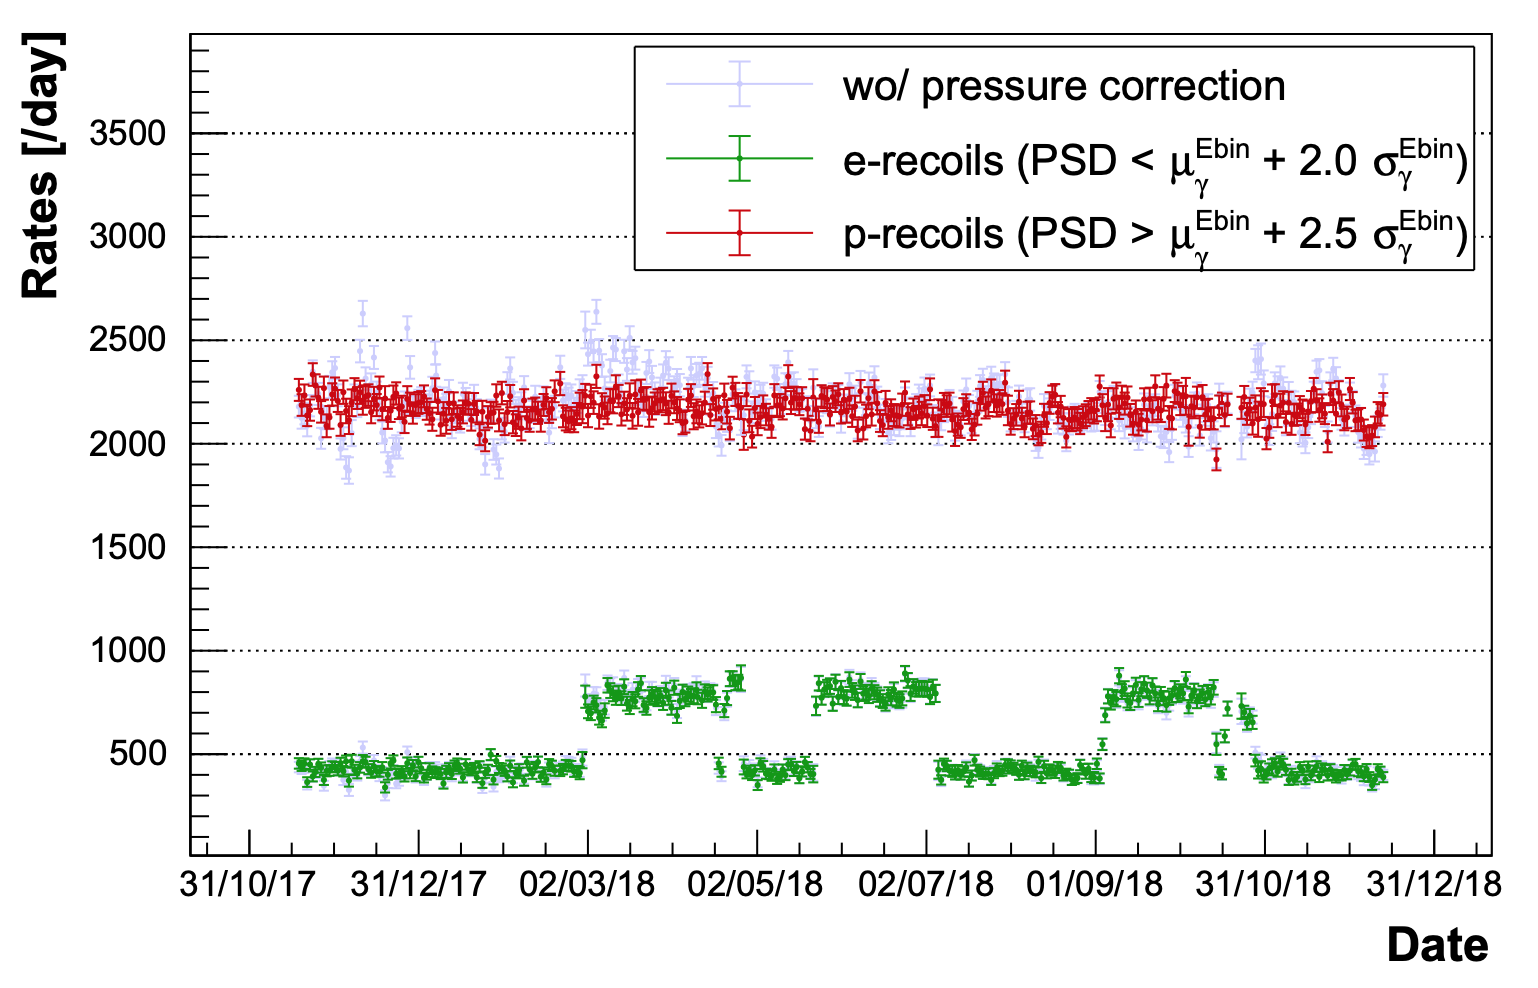
\includegraphics[width=0.8\linewidth]{images/corr_rates_vs_time.png}
  \caption[Évolution des taux de comptage de paires corrélées en fonction du temps]{Évolution des taux de comptage de paires corrélées en fonction du temps. Les points rouges représentent le taux de candidats corrélés identifiés comme protons de recul ($PSD > \mu_\gamma^{PSD} + 2.5 \sigma_\gamma^{PSD}$) tandis que les points verts sont les paires dont les dépôts d'énergie Prompt sont identifiés comme des électrons de recul ($PSD < \mu_\gamma^{PSD} + 2 \sigma_\gamma^{PSD}$). C'est dans cette dernière composante que se loge le signal neutrino. À titre indicatif, le taux de paires corrélées type protons de recul avant correction de la pression est dessiné en bleu. (source : \cite{docdb810})}
  \label{fig:corr_rates_vs_time.png}
\end{figure}

\begin{figure}[h!]
  \centering
  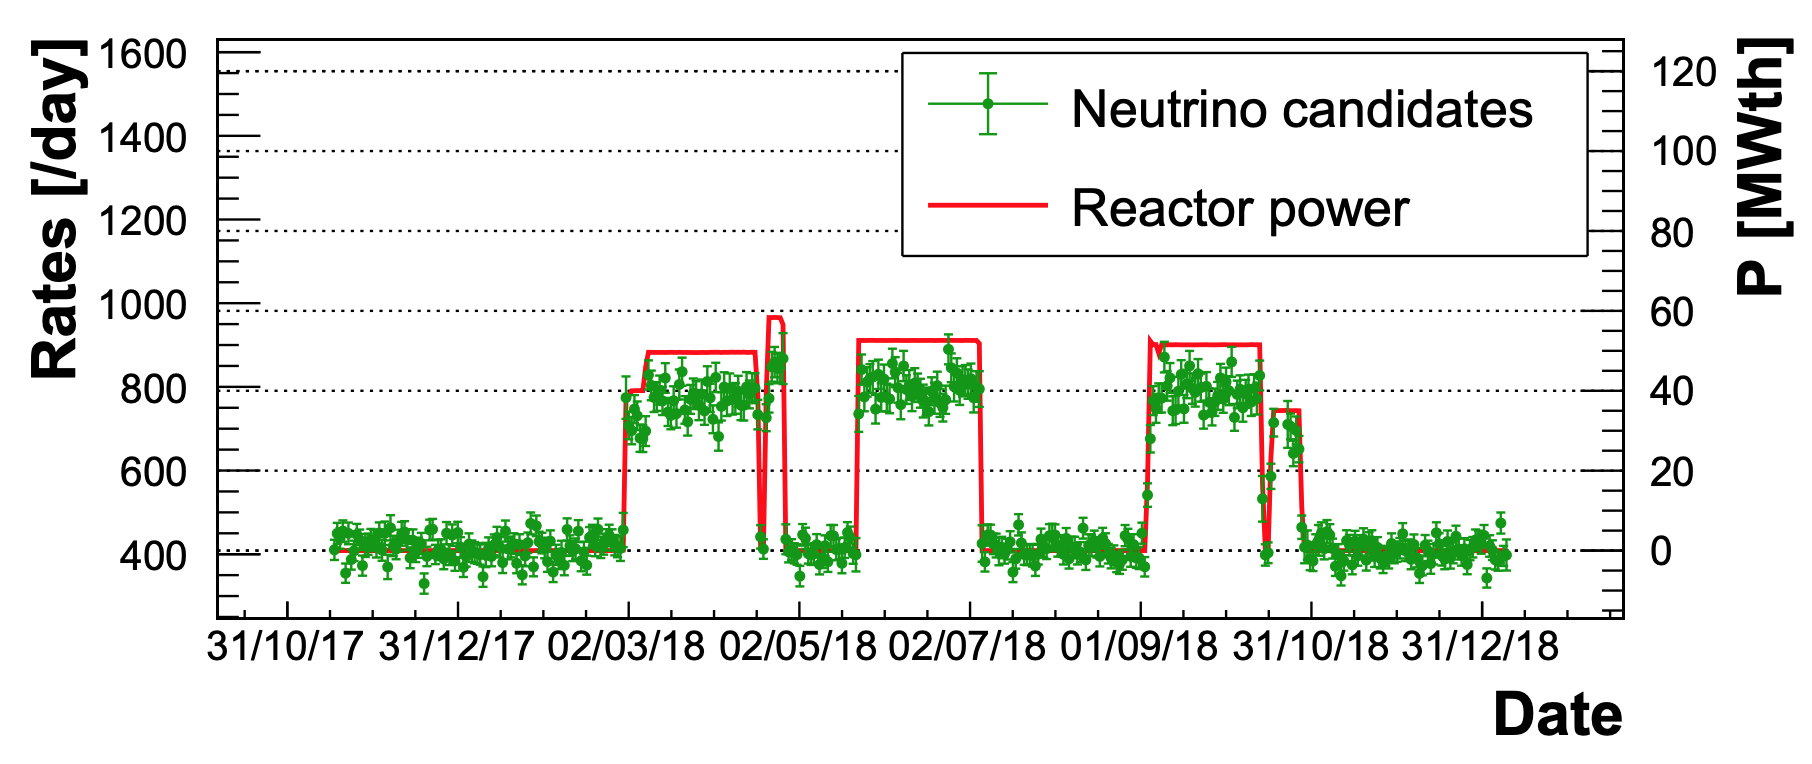
\includegraphics[width=0.7\linewidth]{images/rates_vs_reactor.png}
  \caption[Corrélation entre la puissance réacteur et le taux de candidats neutrinos]{Corrélation entre la puissance réacteur (ligne rouge) et le taux de candidats neutrinos (points verts). Les variations des taux de paires corrélées apparaissent par marches au moment où le réacteur se met en route. (source : \cite{docdb810})}
  \label{fig:rates_vs_reactor.png}
\end{figure}

}

Le rapport signal sur bruit est décisif pour la sensibilité aux paramètres d'oscillation. L'évolution des taux de comptage de paires corrélées en fonction du temps, présentée figure \ref{fig:corr_rates_vs_time.png}, témoigne du caractère vital de l'observable PSD. En effet sans la PSD, le taux de comptage du bruit de fond seul est d'environ $2500$ candidats par jour réduisant le rapport signal sur bruit à environ $0,15$. Avec la coupure PSD, ce rapport est d'environ 1 en moyenne sur tout le spectre neutrino. Après correction des effets de la pression, on distingue clairement les périodes d'arrêt des périodes de fonctionnement du réacteur par les changements brutaux des taux de paires sur la composante électron (voire figure \ref{fig:rates_vs_reactor.png}). Les événements qui s'ajoutent lorsque le réacteur est ON sont les neutrinos. Enfin, la stabilité remarquable des taux de comptage est le \textit{smoking gun} des efforts entrepris pour contrôler la réponse du détecteur. En effet par exemple, si l'échelle en énergie variait significativement, les coupures topologiques auraient une acceptance différente en ON et OFF, alors les taux de candidats IBD présenteraient des variations résiduelles.\\

\afterpage{

\begin{figure}[h!]
\centering

\begin{subfigure}[b]{0.49\textwidth}
\centering
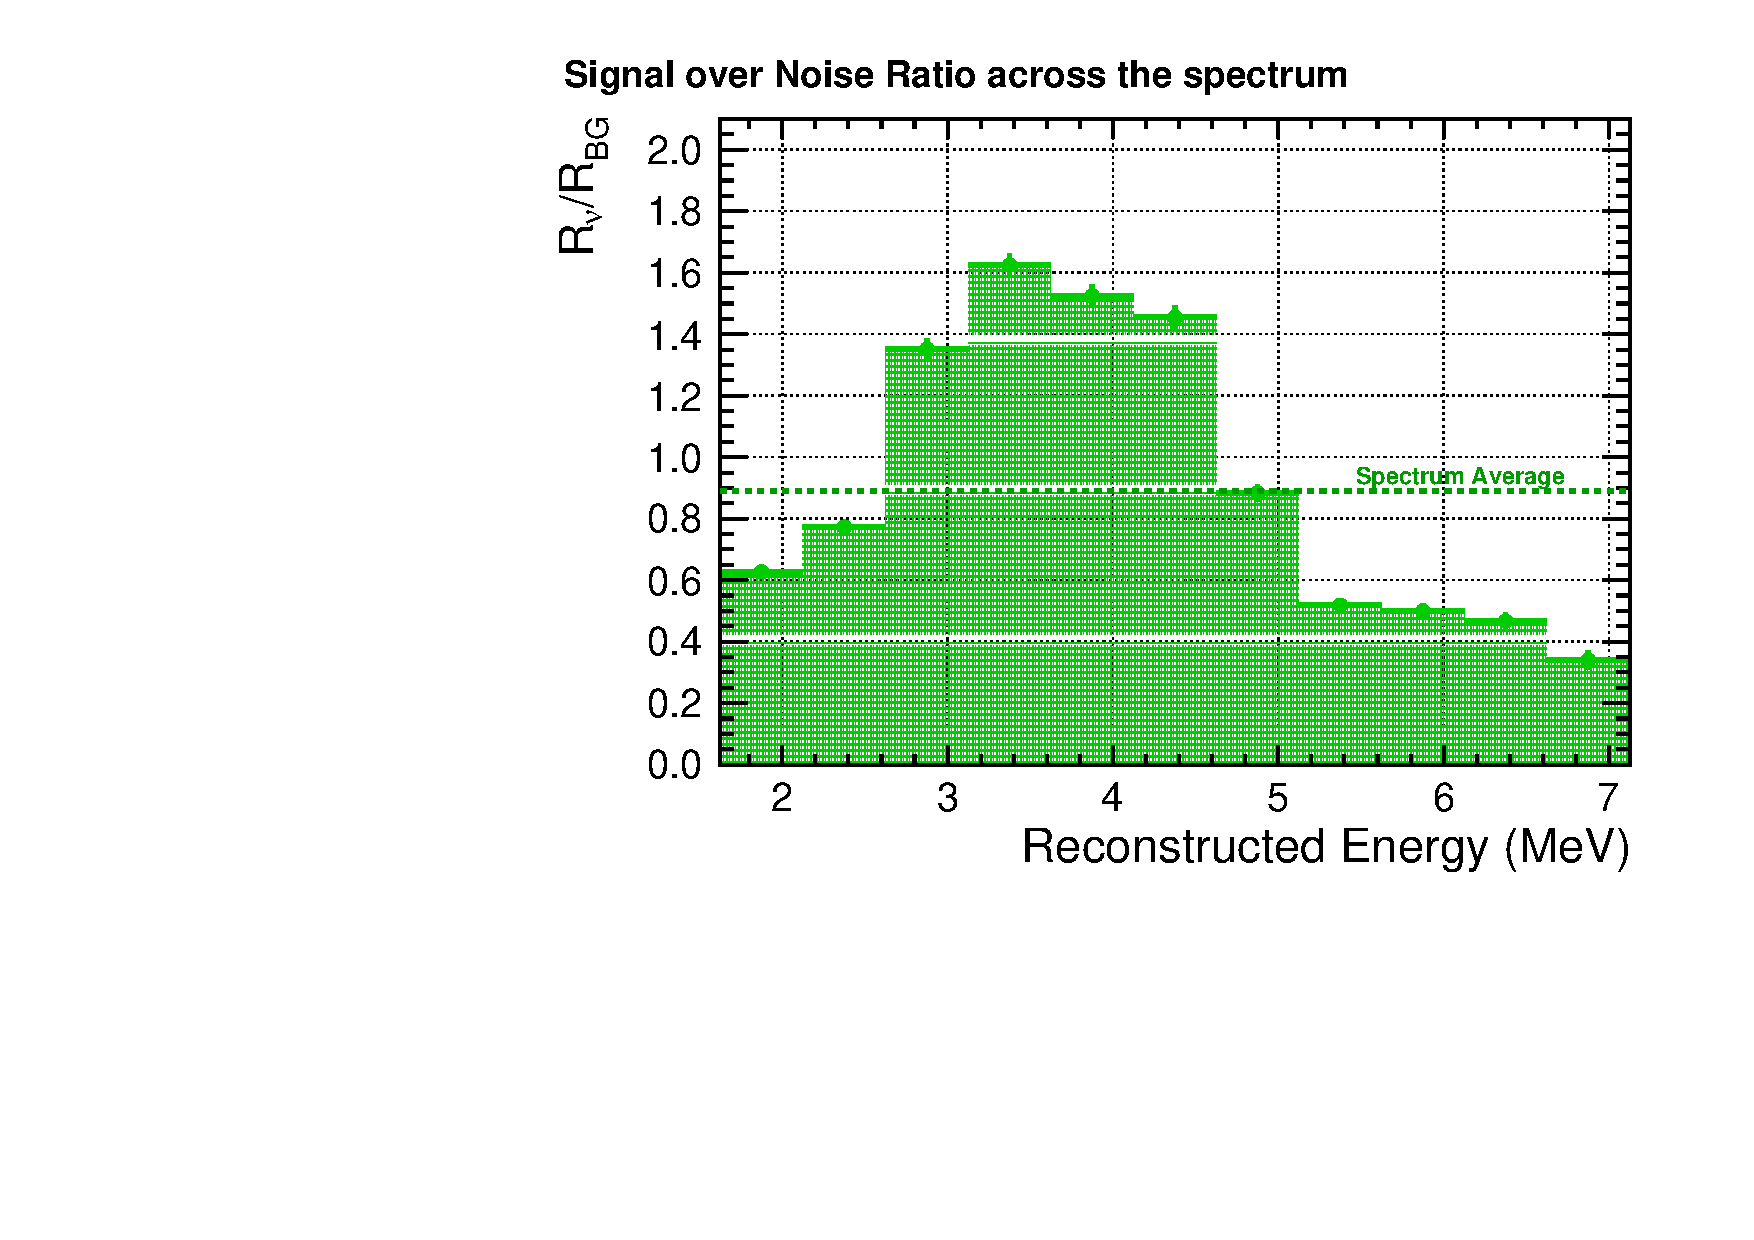
\includegraphics[width=1\textwidth]{images/SNR_spectrum_phase2.pdf}
\caption{}
\label{fig:SNR_spectrum_phase2.pdf}
\end{subfigure}
~ % attention ! space sensitive
\begin{subfigure}[b]{0.49\textwidth}
\centering
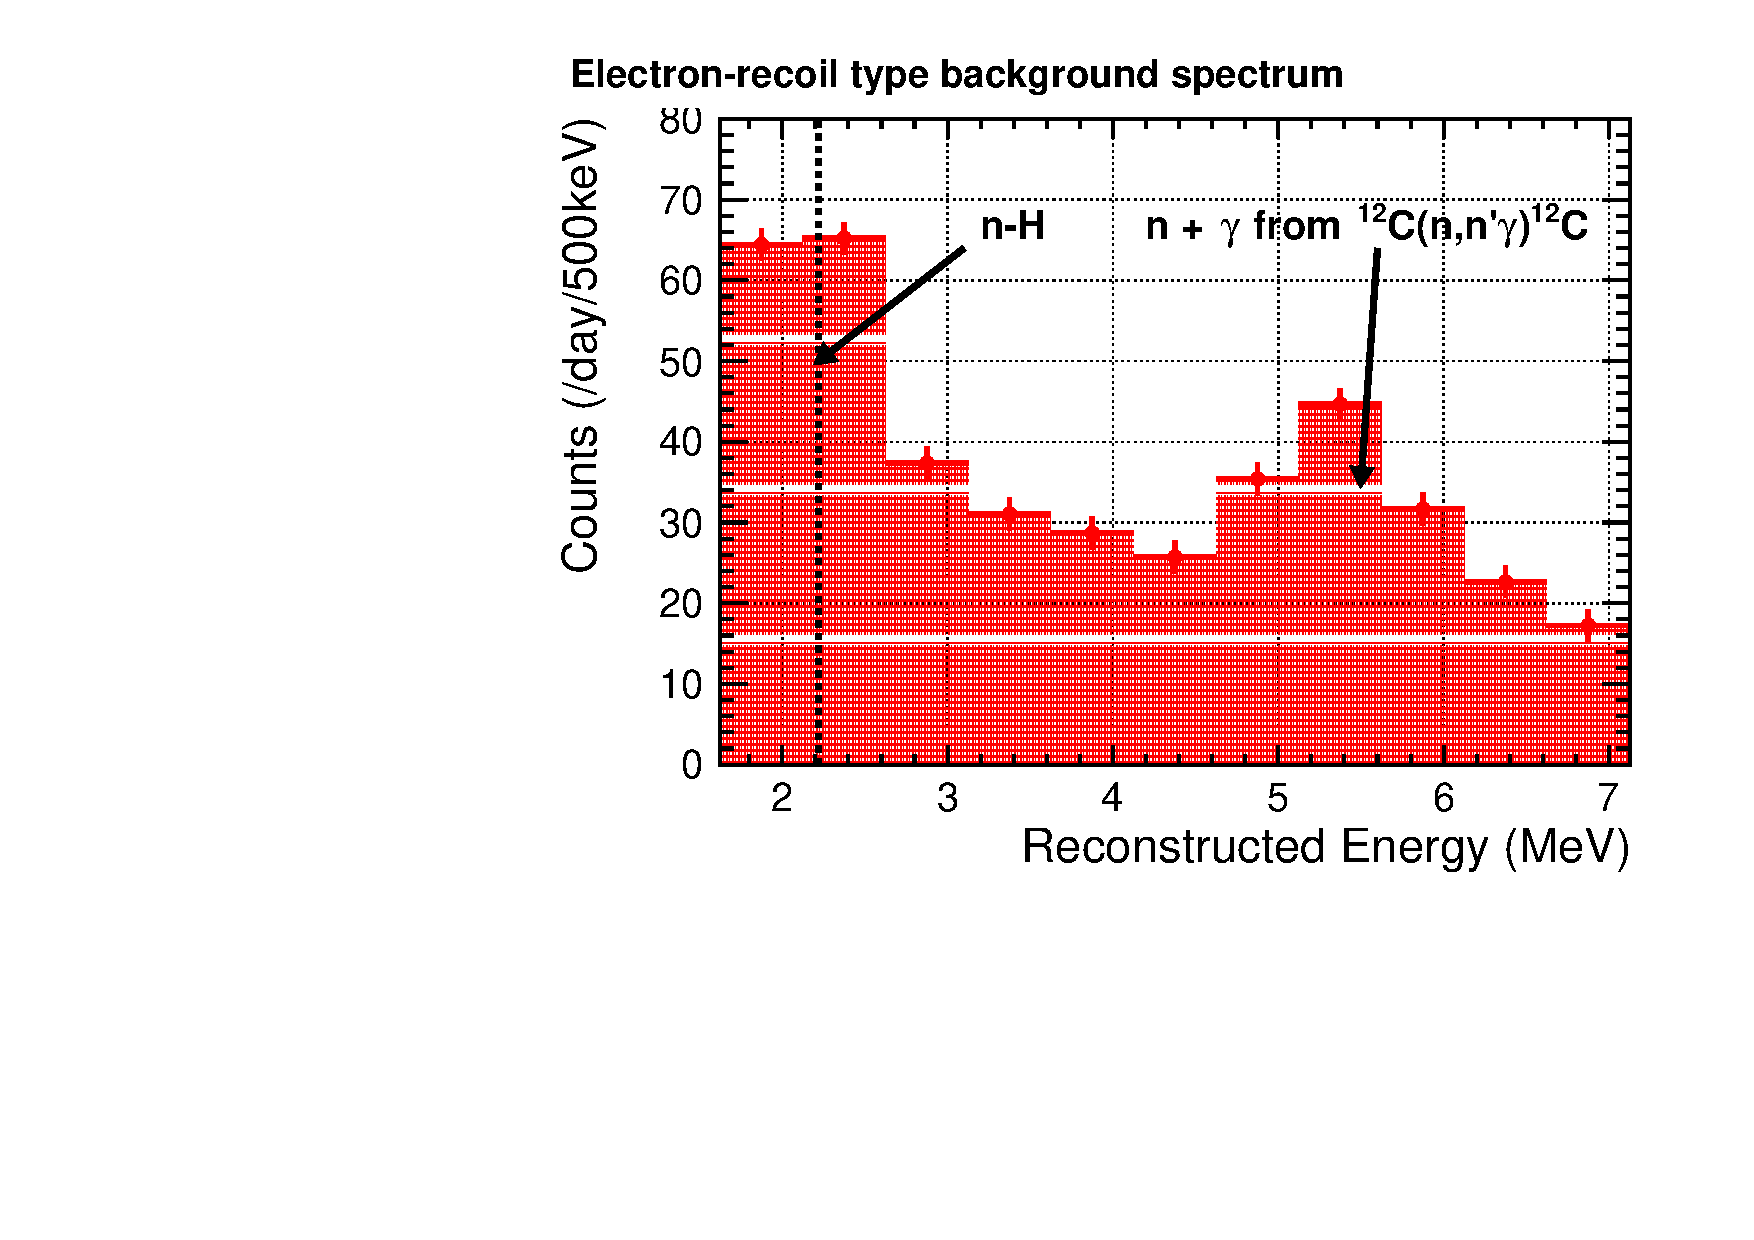
\includegraphics[width=1\textwidth]{images/BG_spectrum_phase2.pdf}
\caption{}
\label{fig:BG_spectrum_phase2.pdf}
\end{subfigure}

\caption[Spectres du bruit de fond et du rapport signal sur bruit]{Rapport signal sur bruit (a) et spectres du bruit de fond type électronique (b). Le spectre de bruit de fond laisse apparaître le pic de capture n-H et celui de la diffusion de neutrons sur $\ce{^{12}C}(n,n'\gamma )\ce{^{12}C}$. La ligne horizontale verte sur (b) représente la valeur du rapport signal sur bruit moyenné sur tout le spectre.}
\label{fig:BG_SNR_spectra}

\end{figure}

}

Le nombre de neutrinos mesuré est de $ (365.7 \pm 3.2_\textrm{stat} ) \SI{}{/\textrm{jour}}$ en phase 2. Comme décrit dans la Section \ref{sec:nu_extraction}, les spectres positron sont reconstruits avec les méthodes d'extraction des taux neutrino dans chaque cellule et chaque bin en énergie reconstruite. L'intensité relative du bruit de fond varie sur une échelle de 0,4 à 1,6, dont la moyenne sur tout le spectre fait 0.9 (voire figure \ref{fig:SNR_spectrum_phase2.pdf}). Le spectre du bruit de fond laisse apparaitre des structures qui témoignent de la nature des événements qui l'ont engendré (cf. figure \ref{fig:BG_spectrum_phase2.pdf}). Tout d'abord, il faut distinguer les deux composantes qui forment cet histogramme : les bruits de fond accidentels et les bruits de fond corrélés. Le spectre des accidentelles n'est en fait dominant que dans le premier bin en énergie: il s'écroule rapidement après $\SI{2}{MeV}$ jusqu'à devenir négligeable devant la composante corrélée. En outre, cette dernière comporte dans un premier temps le pic de capture n-H qui a servi à l'estimation des incertitudes systématiques sur l'échelle en énergie (cf. chapitre \ref{chap:chapitre_energie}). Leur présence signifie que malgré la coupure véto muon, des neutrons parviennent à pénétrer le détecteur pour se faire capturer sur un noyau d'hydrogène. De plus, puisque ces événements font partie de la composante corrélée, les candidats Retardés ont donc été acceptés selon les critères de sélection de la cascade n-Gd. Par conséquent, ces paires corrélées sont probablement dues aux captures successives de deux neutrons différents --- d'abord sur un noyau d'hydrogène puis sur un gadolinium ---  mais issus de la même gerbe cosmique. On pourrait être surpris de constater que l'événement n-H soit détecté avant le n-Gd alors que le temps de capture sur ce dernier est un ordre de grandeur plus bas. En fait, la présence de noyaux de gadolinium est exclusive au volume de la Target, tandis que les milieux hydrogénés abondent dans l'ensemble du détecteur interne: liquide de la Target, du Gamma-Catcher, parois en acrylique ou encore \textit{buffers}. En fait les neutrons détectés dans la fenêtre Retardé voient leurs temps de vie prolongée en diffusant quelques instants en bordure de la Target avant d'y entrer et de se faire capturer par un noyau de gadolinium. Cette supputation a été confirmée en montrant que la distribution des durées Prompt-Retardé est plus étalée qu'une simple capture de neutron n-Gd \cite{docdb293}.\\

La bosse présente à environ $\SI{5.5}{MeV}$ sur la figure \ref{fig:BG_spectrum_phase2.pdf} correspond à la diffusion inélastique de neutrons rapides sur un noyau de Carbone 12:

\begin{equation}
\begin{gathered}
    n + \ce{^{12}C} \rightarrow \ce{^{12}C^*} + n'\\
    \textrm{puis } \ce{^{12}C^*} \rightarrow  \ce{^{12}C} + \gamma(\SI{4.439}{MeV}),
\end{gathered}
\end{equation}

\bigbreak

où le neutron rapide $n'$ a perdu une partie de son énergie cinétique initiale. L'énergie transmise au $\ce{^{12}C}$ est emmagasinée sous forme d'excitation nucléaire, puis dissipée en émettant un gamma de $\SI{4.439}{MeV}$. L'événement Prompt associé à cette réaction est causé par les dépôts d'énergie du gamma et du neutron rapide $n'$, tandis que le Retardé provient de la capture de $n'$ sur un noyau de gadolinium une fois qu'il a thermalisé. Le neutron dépose son énergie en collisionnant avec des protons qui engendrent le processus de scintillation. Cependant l'énergie déposée est très affectée par le quenching donc sa contribution au bilan énergétique gamma + neutron est bien inférieure à son énergie nominale\footnote{Notons que c'est justement parce que l'énergie des neutrons rapides est quenchée que leur PSD est plus haute que celle des électrons (cf Section \ref{seq:scintillation}).}. En définitive, l'énergie de ces événements Prompt est attendue légèrement supérieure à $\SI{4.4}{MeV}$. La position de cette bosse a été confirmée lors de l'étude de la source d'AmBe. En effet, la décroissance du $\ce{^{13}C}$ provoquée par la capture alpha du noyau de béryllium génère un $\ce{^{12}C^*}$ qui produit à son tour un gamma de $\SI{4.4}{MeV}$ :

\begin{equation}
    \alpha + \ce{^{9}Be} \rightarrow \ce{^{13}C} \rightarrow \ce{^{12}C^*} + n.
\end{equation}

\bigbreak

Les candidats Prompt de la source d'AmBe laissent apparaître une structure spectrale similaire à celles observées avec les candidats neutrino \cite{docdb319}. Par ailleurs, les études de PSD des candidats neutrinos ont montré que ces événements sont constitués d'un empilement $\gamma + n$: leur PSD est hybridée \cite{docdb587} (cf. Section \ref{sec:nu_extraction}).\\

Avant d'analyser les distorsions relatives des spectres entre cellules, il convient de vérifier la provenance du signal mesuré. Si les signaux proviennent bien du c\oe ur du réacteur, alors la quantité de neutrinos détectés doit diminuer avec la distance. C'est l'objet de la discussion dans la section suivante.

% TODO : ++ PRECISION neutron rapides en ON ?

\bigbreak

\subsection{Évolution relative du flux de neutrino avec la distance du réacteur}

\afterpage{

\begin{figure}[h!]
  \centering
  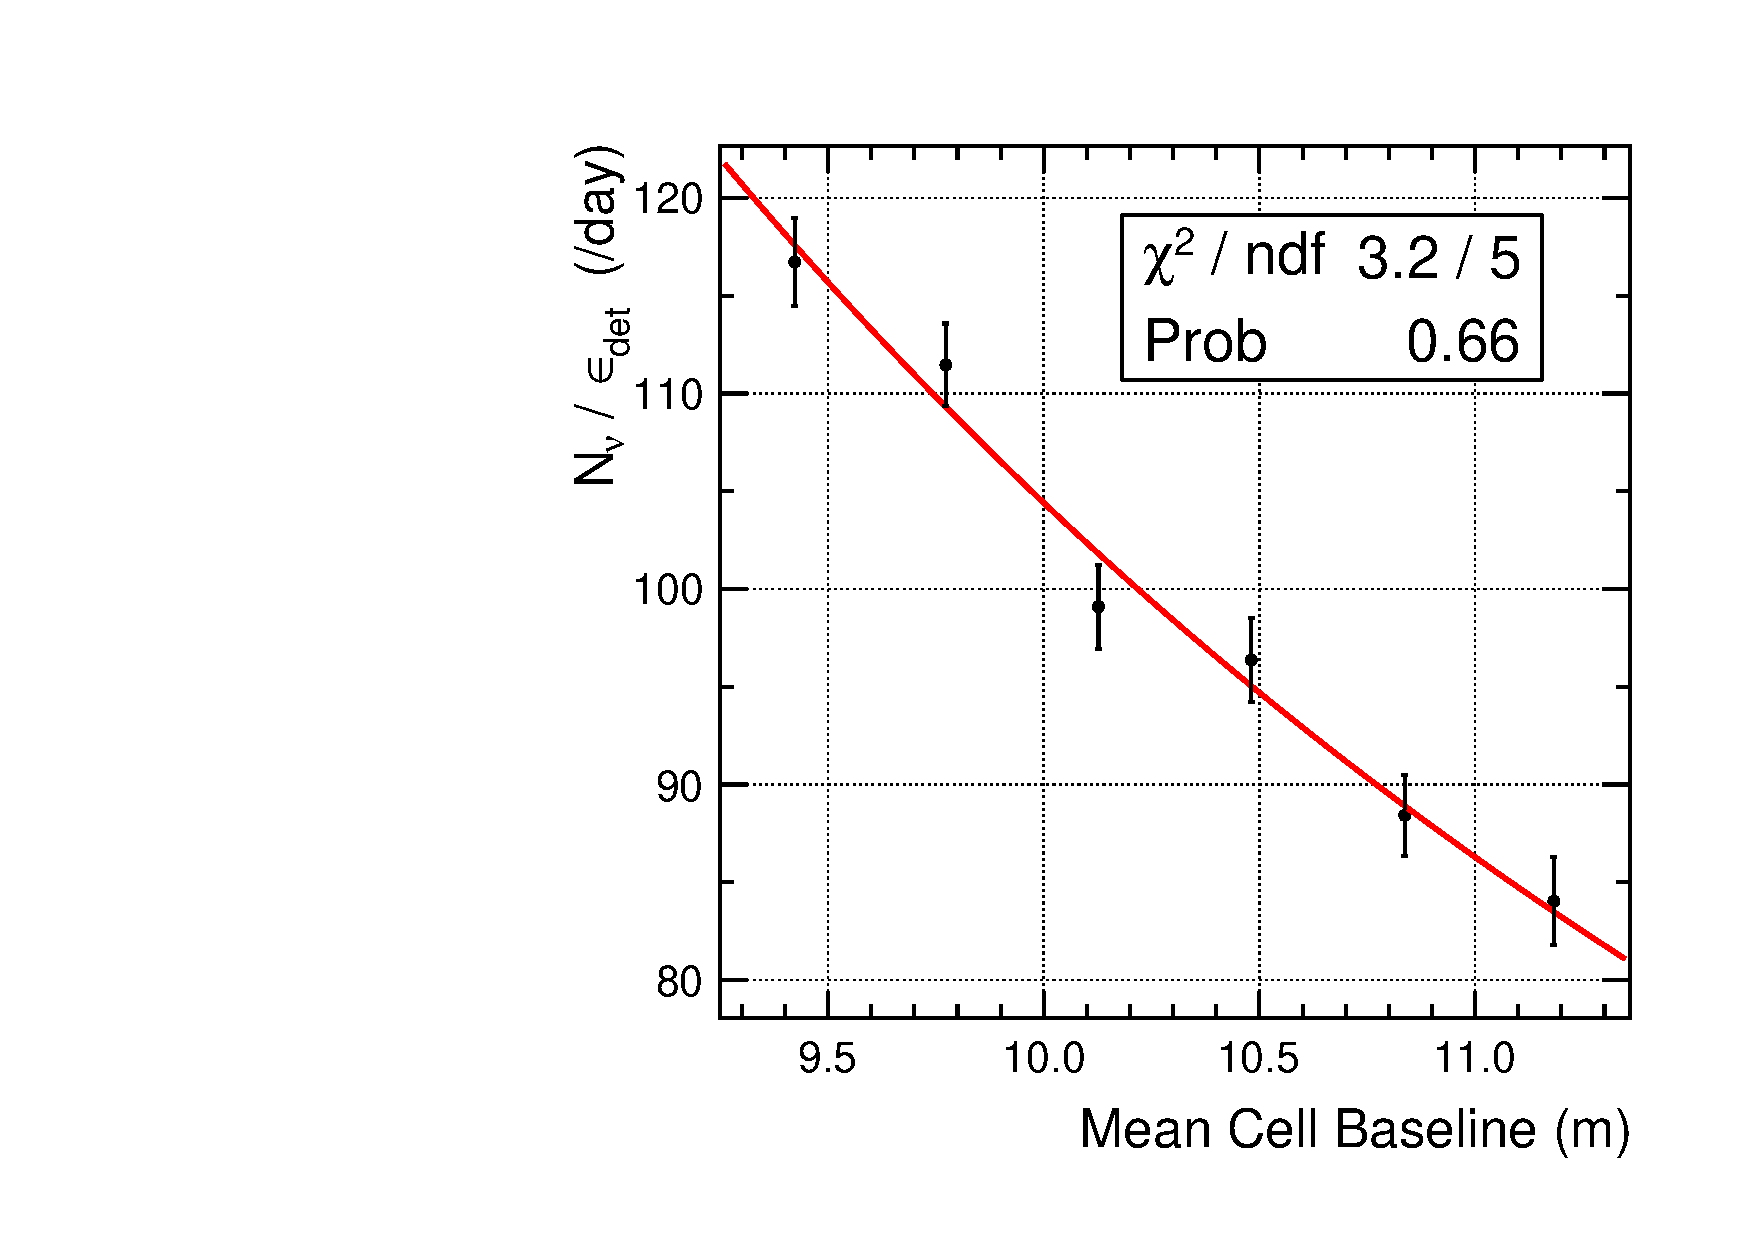
\includegraphics[width=0.7\linewidth]{images/D2_Law.pdf}
  \caption[Évolution du taux de neutrinos détectés avec la distance au c\oe ur du réacteur]{Évolution du taux de neutrinos détectés avec la distance au c\oe ur du réacteur. La courbe rouge correspond à l'ajustement d'un modèle en $1/L^2$. (source : \cite{docdb872})}
  \label{fig:D2_Law.pdf}
\end{figure}

\begin{figure}[h!]
  \centering
  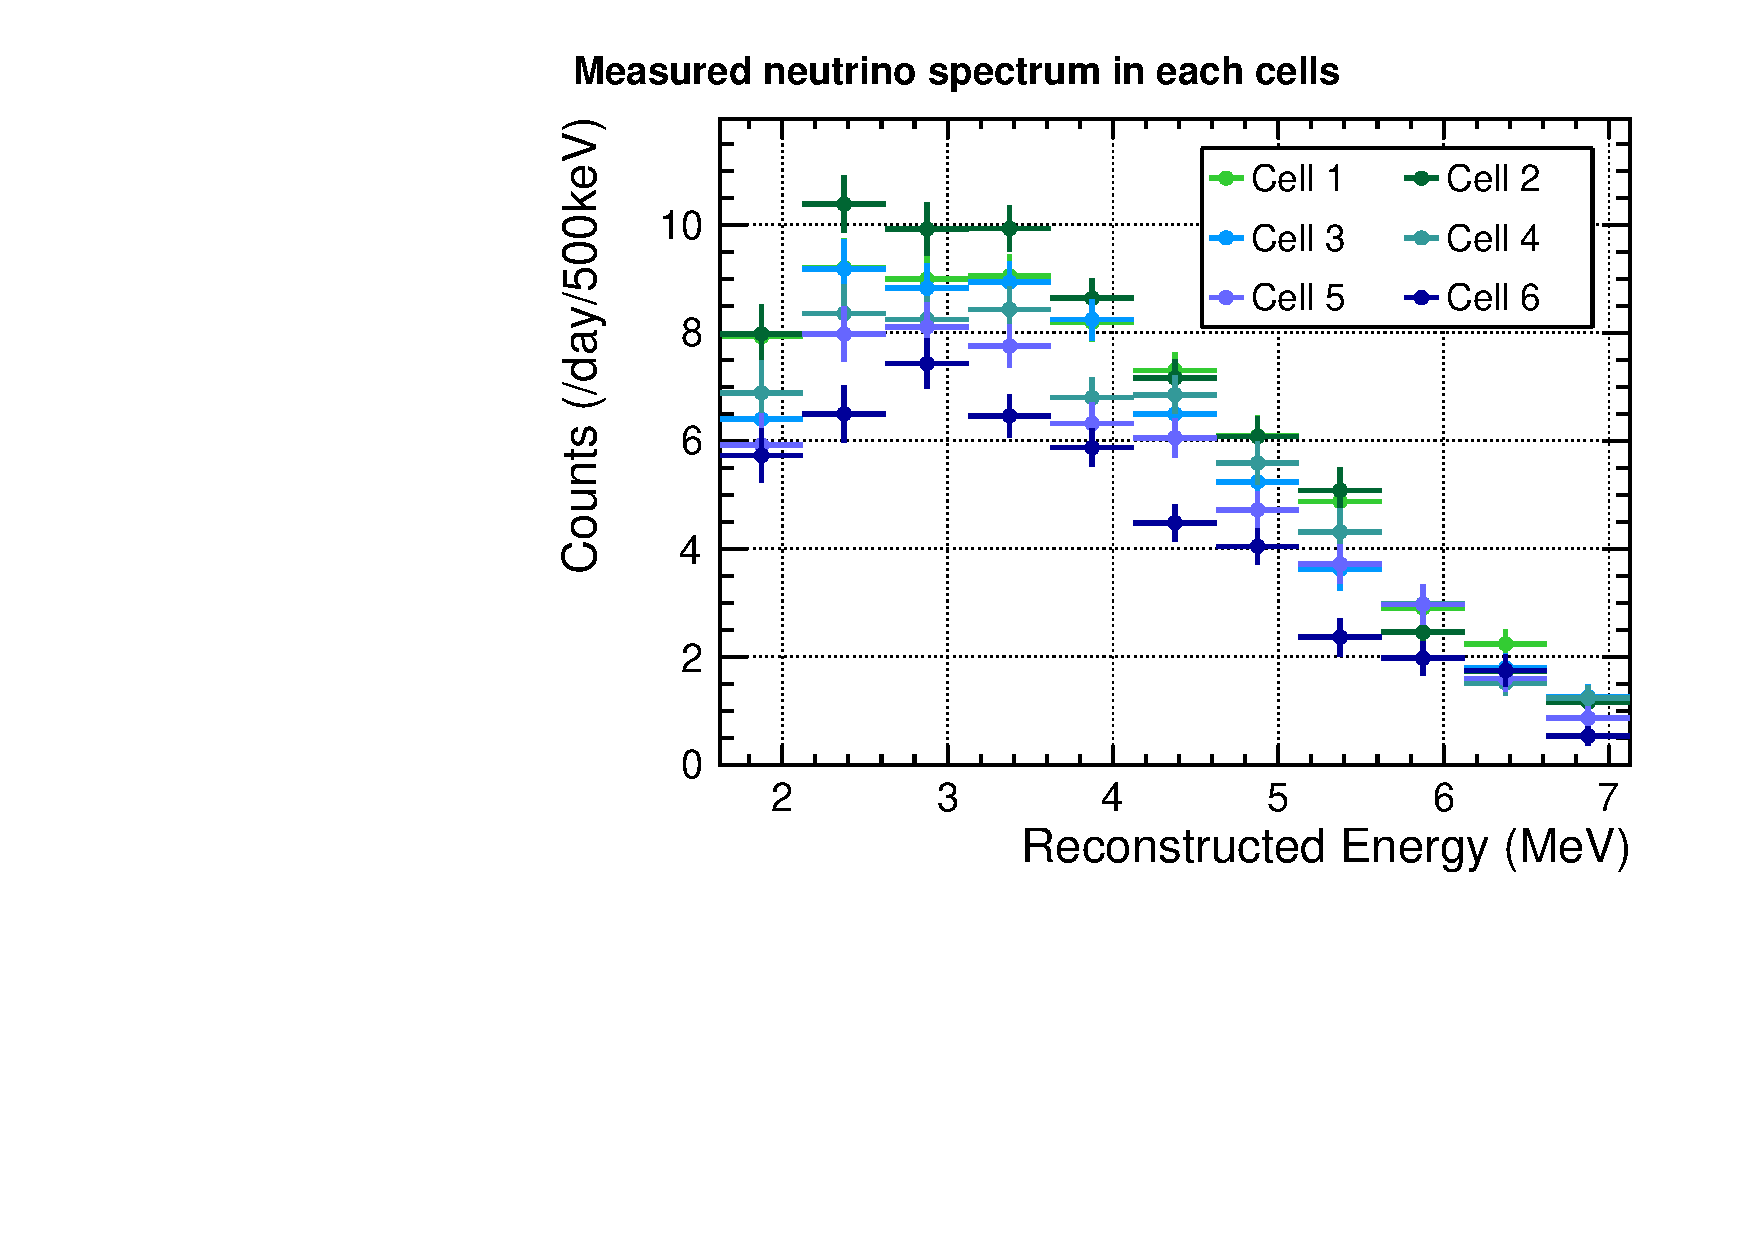
\includegraphics[width=0.9\linewidth]{images/Nu_spectra_phase2.pdf}
  \caption[Spectres positron en énergie reconstruite issu des données de la phase 2]{Spectres positron en énergie reconstruite issu des données de la phase 2.}
  \label{fig:Nu_spectra_phase2.pdf}
\end{figure}

\clearpage

%\begin{table}[h!]
%  \begin{center}
%    \begin{tabular}{|c|c|c|c|}
%    \hline
%      Source & Biais & Incertitude & Corrélation cellule à cellule\\
%      \hline
%      \hline
%      Échelle en énergie & $- 1.5 \%$ & $\pm 1.1 \%$ & $100 \%$ \\
%      \hline
%      Échelle en énergie & N.A. & $\pm 0.5 \%$ & $0 \%$ \\
%      \hline
%      Normalisation & Cellules 1 et 6 : $\times 0.909$ & \multirow{2}{*}{$\pm 1.2 \%$} & \multirow{2}{*}{$0 \%$}\\
%      $(V_\textrm{cell}, C_\textrm{Gd}^\nu)$ & Cellules 2,3,4,5 : $\times 0.931$ & & \\
%      \hline
%    \end{tabular}
%  \end{center}
%  \caption[Liste des incertitudes systématiques utilisées pour les résultats de Moriond 2019]{Liste des incertitudes systématiques utilisées pour les résultats de Moriond 2019. Un biais sur l'échelle en énergie commun à toutes les cellules avait été mesuré, c'est pourquoi il est corrigé. Il s'agissait d'un bug dans la façon de récupérer les charges collectées dans chaque cellule. (source : \cite{docdb840})}
%    \label{tab:v33_syst}
%\end{table}

}

Tester l'évolution du taux de neutrinos détectés en fonction de la distance de propagation permet à la fois de vérifier que le réacteur est bien la source du signal, et que l'efficacité de détection est bien décrite par la simulation. Le flux de neutrinos qui interagissent dans le volume cible doit suivre une loi en $1/L^2$ où $L$ est la distance au c\oe ur. Les 6 cellules ont des géométries identiques, donc le nombre de neutrinos détectés par cellule doit décroitre en $1/L^2$. Cependant l'efficacité de détection n'est pas homogène et doit être corrigée en amont. Cette dernière est déterminée avec la simulation calculant le rapport du nombre de neutrinos identifiés dans la cellule $i$ ($N^\nu_\textrm{det}(i)$) sur le nombre de neutrinos qui ont interagi dans cette cellule ($N^\nu_\textrm{int}(i)$) :

\begin{equation}
    \varepsilon_i^{MC} \doteq N^\nu_\textrm{det}(i) /N^\nu_\textrm{int}(i)
\end{equation}

\bigbreak

De plus, puisque cette valeur n'est connue que dans le MC, les facteurs de corrections quantifiant le désaccord entre les données et la simulation doivent être appliqués (cf. Tableau \ref{tab:data_mc_gd_fraction_ratios}). Le nombre de neutrinos corrigé $N^{\nu *}_\textrm{Data}$ s'exprime en définitive comme :

\begin{equation}
      N^{\nu *}_\textrm{Data} = \frac{N^{\nu}_\textrm{Data}}{\varepsilon_i^{MC} \times \left<C_\textrm{Retardé} \right>_{\textrm{cells},z} \times C^\nu_\textrm{Gd}(i)}
\end{equation}

\bigbreak

L'ajustement d'une courbe $C/L^2$, où C est un paramètre libre, est présenté sur la figure \ref{fig:D2_Law.pdf}. Le $\chi^2$ obtenu a une p-value de 66 \%, montrant la compatibilité des données avec l'hypothèse que le signal neutrino provient du réacteur. Le bras de levier en $L$ étant cependant faible, il serait intéressant de faire un fit en $L^\alpha$ pour voir si $\alpha=2$ est effectivement préféré.

\bigbreak


\subsection{Spectres neutrinos en phase 2}

%\afterpage{
%
%\begin{figure}[h!]
%  \centering
%  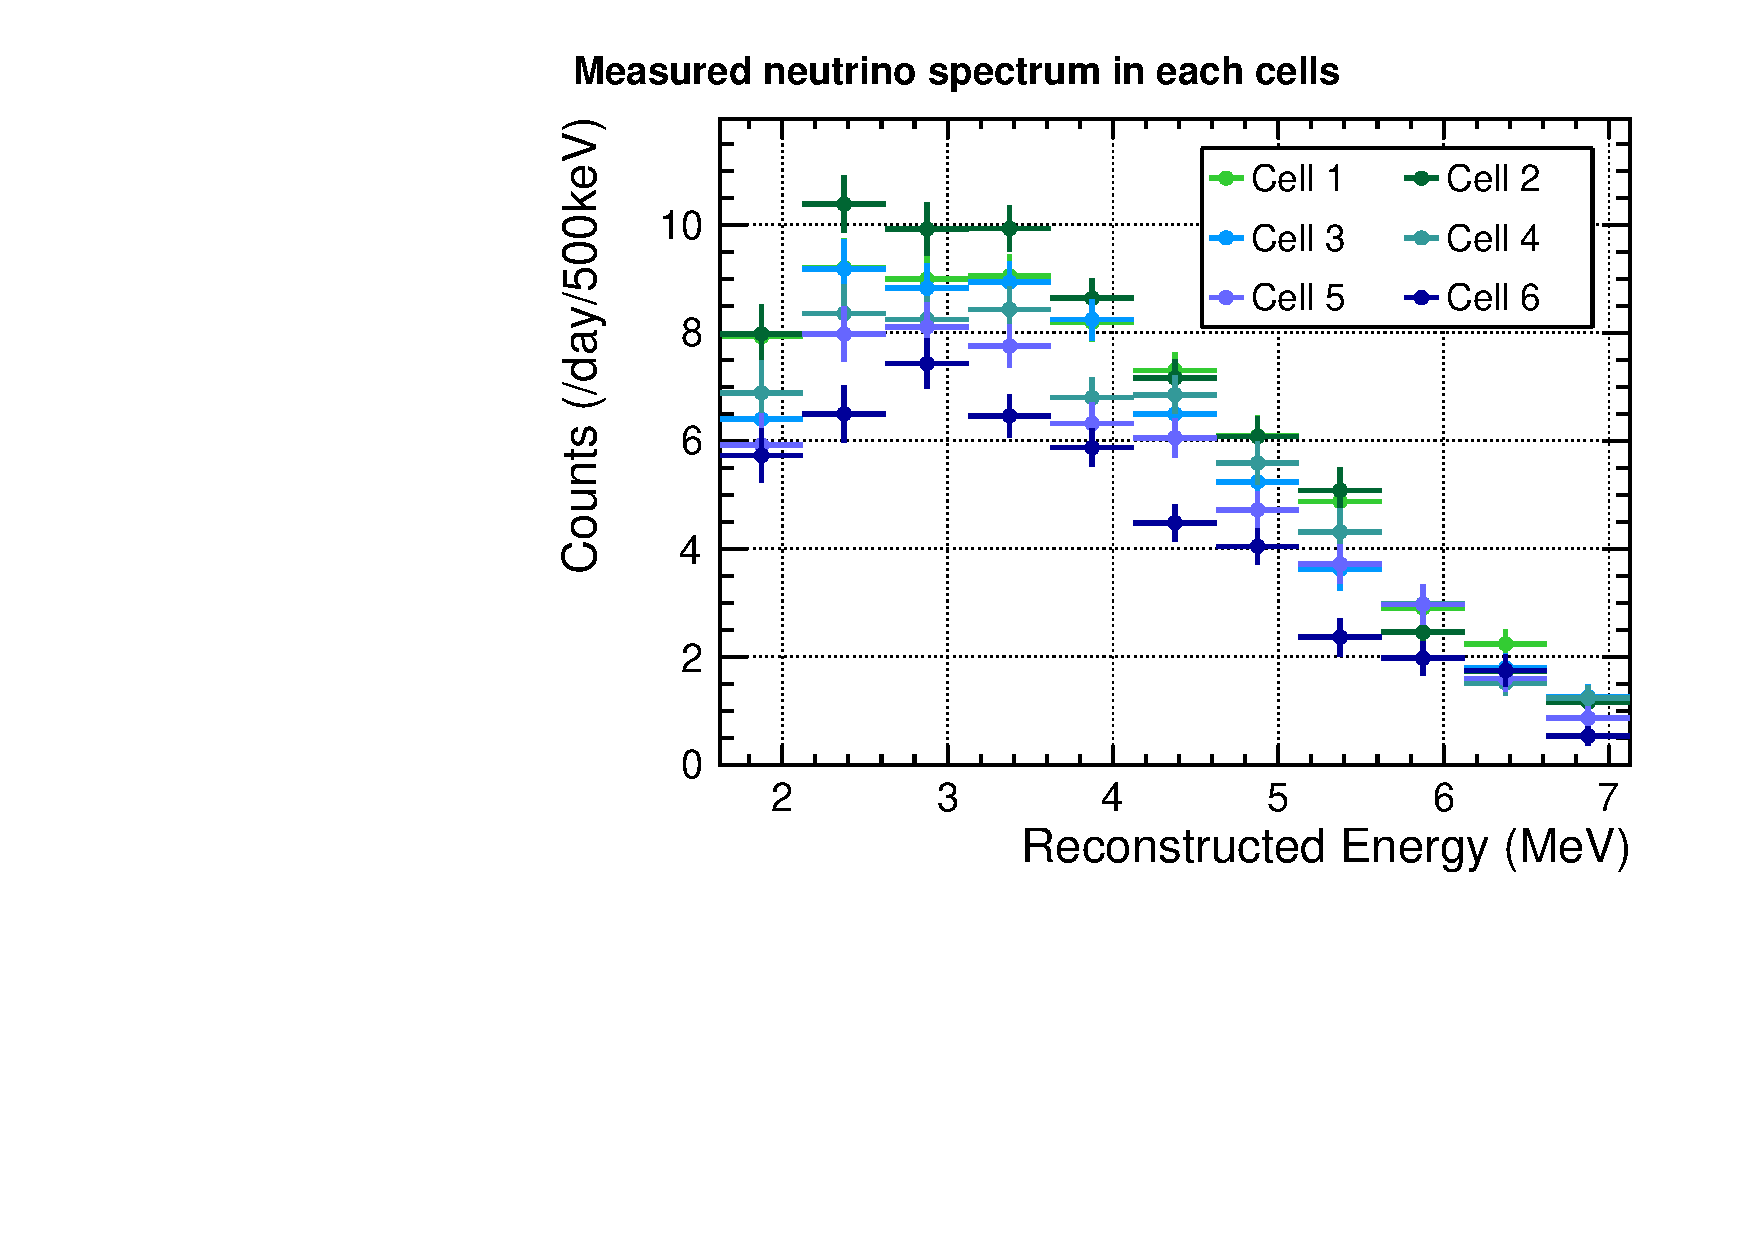
\includegraphics[width=0.8\linewidth]{images/Nu_spectra_phase2.pdf}
%  \caption[Spectres neutrino mesurés dans chaque cellule en phase 2]{Spectres neutrino mesurés dans chaque cellule en phase 2.}
%  \label{fig:Nu_spectra_phase2.pdf}
%\end{figure}
%
%}

La divulgation des spectres neutrinos marque le point de non-retour du développement des outils d'analyse. En effet en vertu du principe d'analyse en aveugle\footnote{Plus souvent appelé \og \textit{blind analysis} \fg{}.}, les études sur la calibration, extraction des spectres, estimation des systématiques ou encore analyse statistique doivent être bloquées et prêtes à l'emploi afin d'éviter toute forme de biais  \og \textit{post-hoc, ergo propter hoc} \fg{} (après cela, donc à cause de cela), c'est-à-dire d'éviter de modifier les spectres par des corrections sur les outils d'analyse après avoir vu les résultats. En pratique cependant, les outils d'analyse sont sur une voie d'amélioration constante, donc les prochaines données phase 2 bénéficiant des dernières améliorations (par exemple calibration, ou encore efficacité de détection...) ne bénéficieront pas de ce cachet.\\

% Les spectres sont présentés sur la figure \ref{fig:Nu_spectra_phase2.pdf}: ce sont ces données qui ont été utilisées pour produire les résultats présentés à Moriond 2019. La version de calibration qui a été utilisée lors de cette analyse est cependant différente de celle présentée dans le chapitre \ref{chap:chapitre_energie}. La simulation déviait des données à hauteur de $-1.5 \%$ à partir de $\sim \SI{1.5}{MeV}$ sur l'échelle en énergie. Ce biais était en fait dû à un \textit{cut off} sur les très basses charges récoltées par les PMs. Ce problème est corrigé aujourd'hui. Le bilan d'erreurs systématiques choisi à l'époque est présenté sur le Tableau \ref{tab:v33_syst}.\\

La méthode d'extraction des spectres par soustraction directe du bruit de fond a été exploitée pour générer les taux de comptage neutrino dans chaque bin en énergie. Il a été choisi de se cantonner aux 11 premiers bins en énergie, car en deçà d'un certain taux de comptage neutrino, les biais de l'estimateur deviennent non négligeables : la valeur du biais grandit en $\propto 1/N$ où $N$ est le taux de comptage neutrino (cf. Section \ref{sec:nu_extraction}). Cela signifie qu'à un certain point, le décalage induit par l'estimateur devient non négligeable devant l'erreur statistique.\\

Ces spectres forment le point de départ de l'analyse statistique décrite dans le chapitre \ref{chap:chapitre_stat}. Ils interviennent dans les $\chi^2$ via les termes en $D_{cb}$. La section suivante est consacrée à l'interprétation de ces résultats.

% TODO : Section chap analyse biais de la methode d'extraction

\bigbreak

\section{Analyse des distorsions relatives des spectres}

Comme mentionné dans le chapitre \ref{chap:chapitre_stat}, il a été choisi de mener l'analyse d'oscillation en s'affranchissant de toute prédiction extérieure des spectres. Les $\chi^2$ utilisés par Saclay (cette thèse) et Grenoble pour l'analyse de la phase 2 sont respectivement :

\begin{equation}
    \begin{gathered}
        \chi^2 = \sum_{c,b} \sum_{c',b'} \left(D_{cb} - \phi_{b} M_{cb}\right) \left(V^{-1}_\textrm{cov}\right)_{cbc'b'} \left(D_{c'b'} - \phi_{b'} M_{c'b'}\right)\\
        \chi^2 = \sum_{c,b} \left(\frac{D_{cb} - \phi_{b} M_{cb}}{\sigma^\textrm{stat}_{cb}}\right)^2 + \sum_c \left( \frac{\alpha^{NU}_c}{\sigma^{NU}_c} \right)^2 + \sum_c \left( \frac{\alpha^{EU}_c}{\sigma^{EU}_c} \right)^2 + \left( \frac{\alpha^{EC}}{\sigma^{EC}} \right)^2,
    \end{gathered}
\end{equation}

\bigbreak

où $\phi_b$ sont des paramètres libres, $D_{cb}$ et $M_{cb}$ les taux de comptage des spectres dans les données et la simulation respectivement, $V^{-1}_\textrm{cov}$ la matrice de covariance inverse et $\alpha^X$ les paramètres de nuisance. À chaque hypothèse testée, la méthode de Saclay se contente de minimiser le $\chi^2$ avec les paramètres $\phi_b$ tandis que la méthode de Grenoble minimise le $\chi^2$ avec $\phi_b$ et les paramètres de nuisance $\alpha^X$. Les deux analyses ont été menées en parallèle en guise de validation croisée. Les deux résultats sont présentés et comparés dans les sous-sections suivantes.

\bigbreak

\subsection{Mise à l'épreuve du modèle standard}

\afterpage{

%
\begin{figure}[h!]
  \centering
  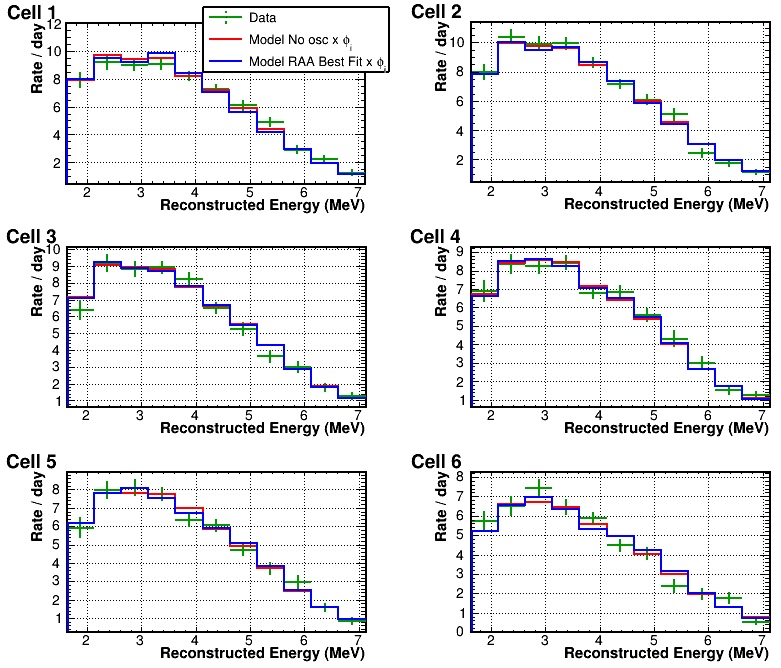
\includegraphics[width=0.8\linewidth]{images/DatavsModel_NoOsc_RAA_Spectra.png}
  \caption[Comparaison entre les spectres mesurés $D_{cb}$ avec le modèle ajusté $\phi_bM_{cb}$]{Comparaison entre les spectres mesurés $D_{cb}$ (vert) et les modèles ajusté $\phi_bM_{cb}$ : sans oscillation en rouge, et en considérant un neutrino stérile avec les paramètres du \textit{best-fit} de la RAA en bleu.}
  \label{fig:Delta_spectra.pdf}
\end{figure}

\begin{figure}[h!]
   \begin{minipage}[c]{.49\linewidth}
      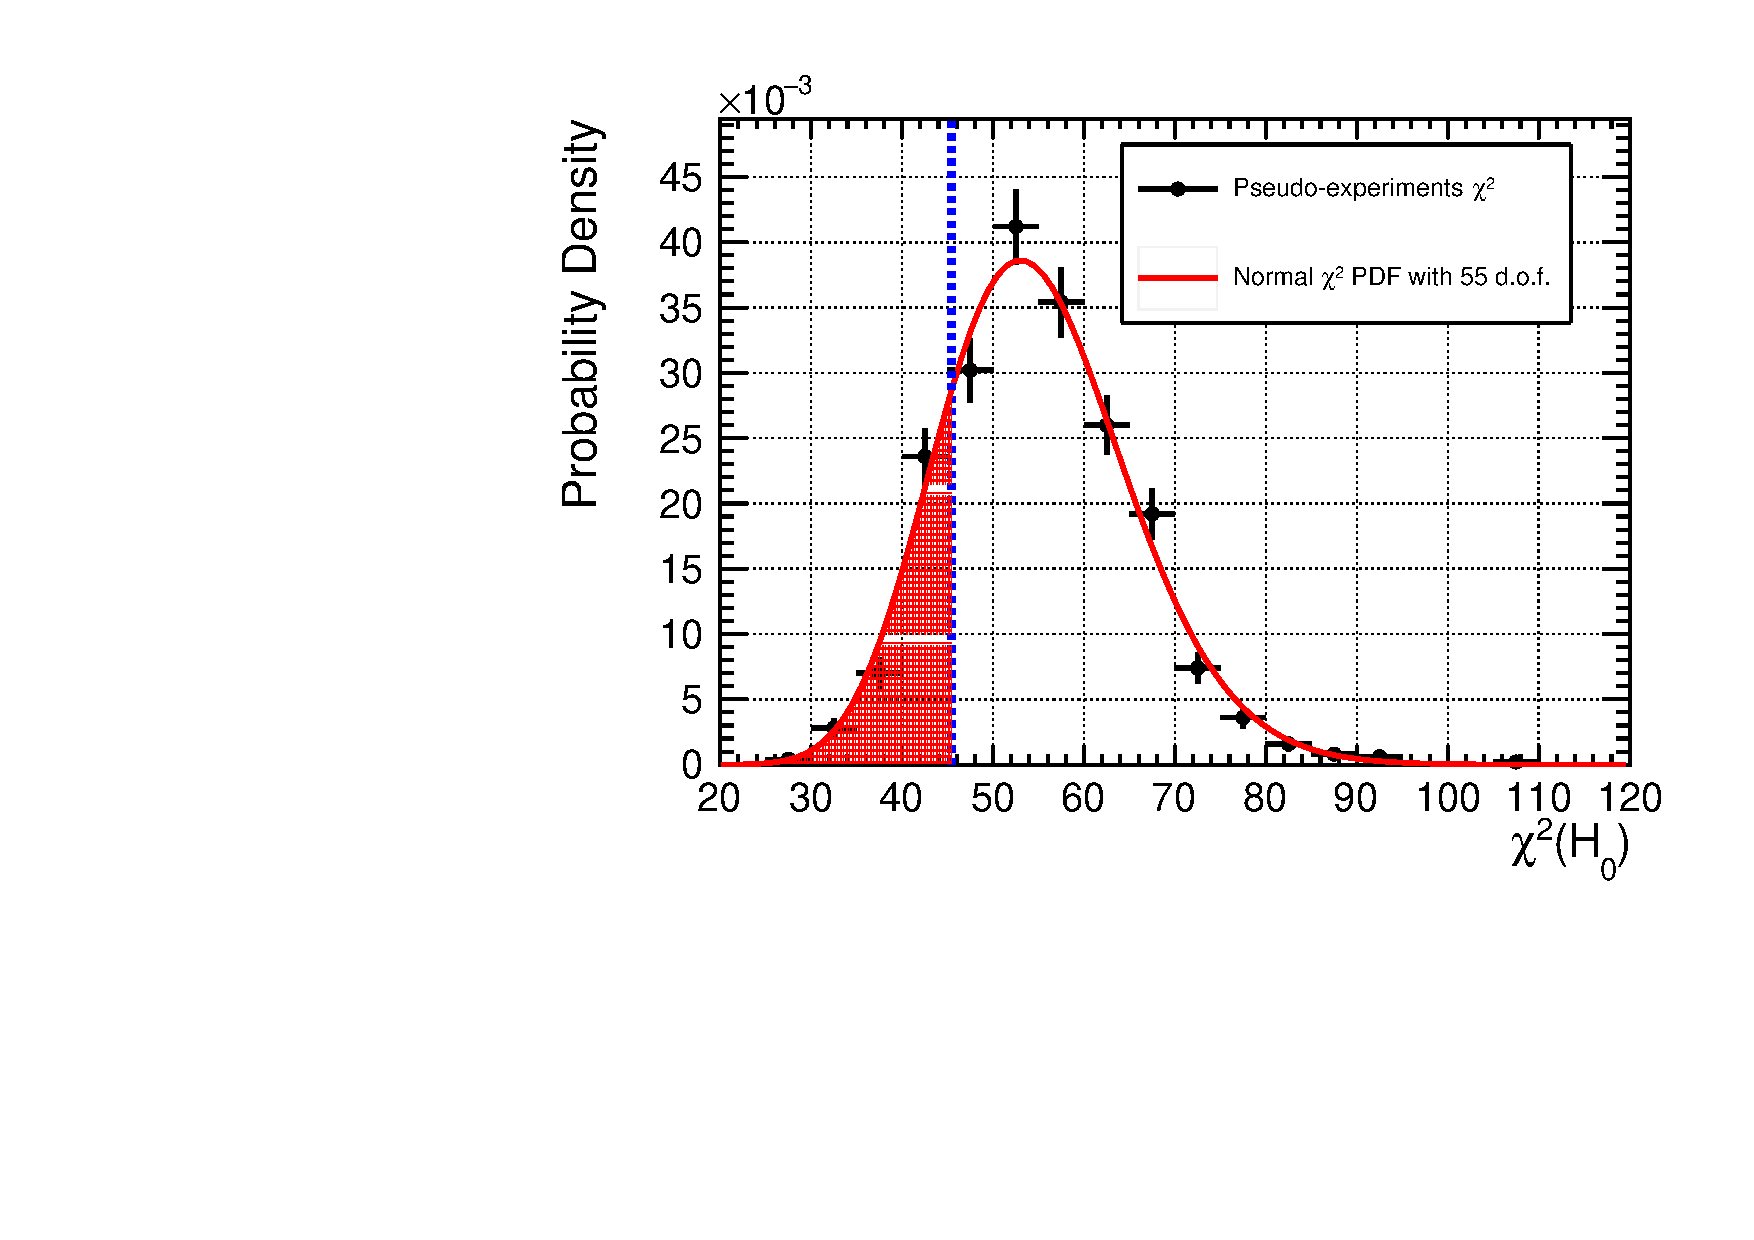
\includegraphics[width=1\linewidth]{images/null_hypothesis_chi2.pdf}
      \caption[Comparaison de la valeur de $\chi^2_{H_0}$ des données avec les pseudo-expériences]{Comparaison de la valeur de $\chi^2_{H_0}$ des données avec les pseudo-expériences. Les $\chi^2_{H_0}$ suivent une loi normale à $66 - 11$ degrés de liberté (courbe rouge). Les résultats des pseudo-expériences (noir) se montrent en parfait accord avec cette hypothèse. La ligne verticale bleue est le $\chi^2_{H_0}$ des données, sa \textit{p-value} est de : $82 \%$.}
  \label{fig:null_hypothesis_chi2.pdf}
   \end{minipage} \hfill
   \begin{minipage}[c]{.49\linewidth}
      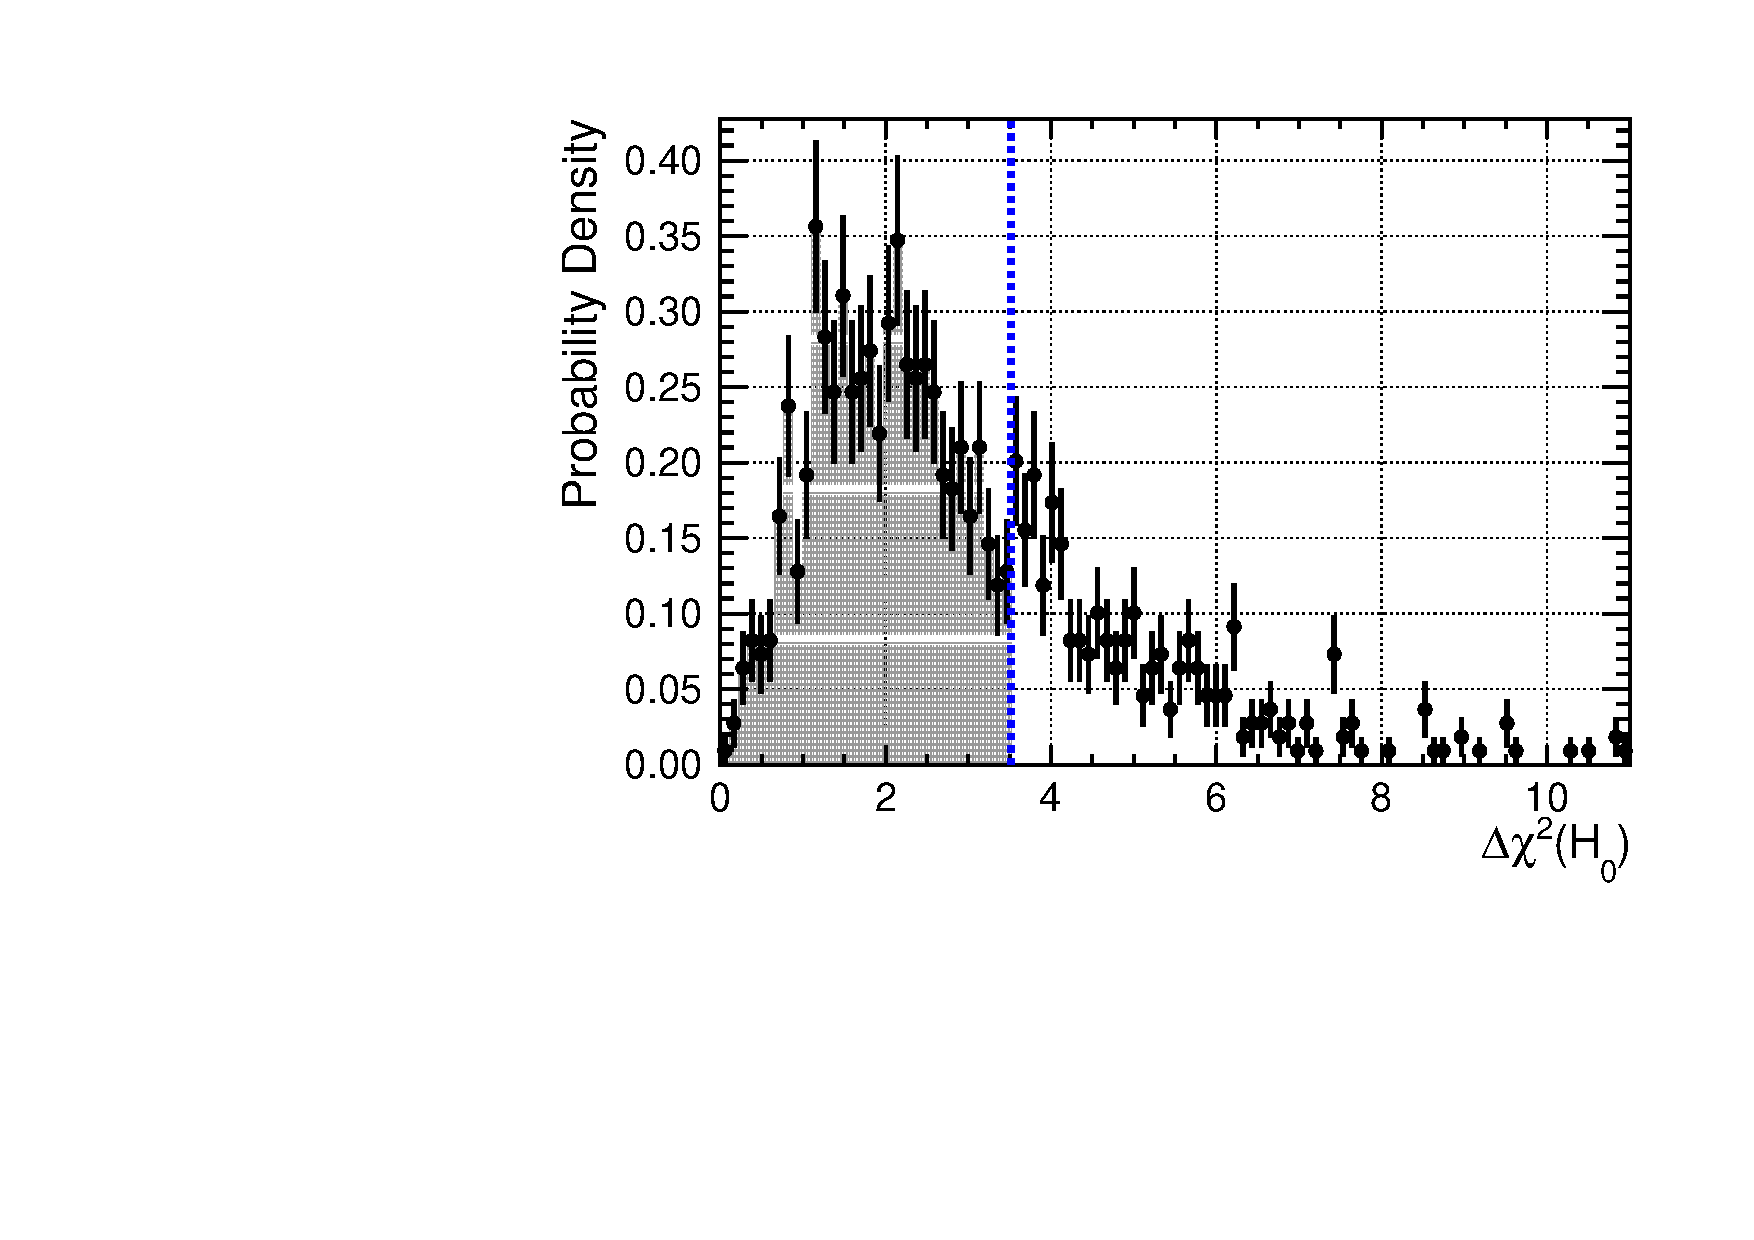
\includegraphics[width=1\linewidth]{images/null_hypothesis_delta_chi2.pdf}
      \caption[Comparaison de la valeur de $\Delta\chi^2_{H_0}$ des données avec les pseudo-expériences]{Comparaison de la valeur de $\Delta\chi^2_{H_0}$ des données avec les pseudo-expériences. Contrairement aux $\chi^2_{H_0}$, les distributions de $\Delta\chi^2_{H_0}$ ne suivent pas des lois normales. La PDF des $\Delta\chi^2_{H_0}$ est déterminée à l'aide de pseudo-expériences (noir). La \textit{p-value} associé au $\Delta\chi^2_{H_0}$ mesuré avec les vraies données est de $31 \%$.}
    \label{fig:null_hypothesis_delta_chi2.pdf}
   \end{minipage}
\end{figure}

\clearpage

}

Puisque le Modèle Standard ne considère que 3 saveurs de neutrinos, ce postulat est désigné comme l'Hypothèse nulle ($H_0$). C'est le premier scénario qui a été testé en étudiant les distorsions relatives des spectres positron.  Les valeurs de $\Delta_{cb} = (D_{cb} - \phi_b M_{cb})$ qui interviennent dans les $\chi^2$ sont tracées sur la figure \ref{fig:Delta_spectra.pdf}. La bande grise indique la déviation standard ($1\sigma$) de $\Delta_{cb}$ estimée en générant des pseudo-expériences. Pour effectuer ce test statistique, la valeur absolue du $\chi^2$ est comparée avec sa loi de distribution associée et une \textit{p-value} en est déduite. Bien qu'\textit{a priori} le $\chi^2$ doive suivre une loi normale à $66(\textrm{cells}\times\textrm{Ebins}) - 11(\phi_b) = 55$ degrés de liberté, les distributions de $\chi^2$ ont été construites avec des pseudo-expériences. La figure \ref{fig:null_hypothesis_chi2.pdf} montre que la \textit{p-value} associée aux données est de  82 \%. Cette valeur signifie que 82 \% des pseudos-expériences ont un $\chi^2$ supérieur à celui des données. Par ailleurs, la valeur due $\Delta\chi^2$ a été mise à l'épreuve. Elle donnée par la différence entre le $\chi^2$ de l'Hypothèse nulle et celui du meilleur ajustement selon  $\Delta m_{14}^2$ et $\textrm{sin}^2\left(2\theta_{14}\right)$ : $\chi^2_\textrm{best-fit}$. Cette fois, la \textit{p-value} doit être déduite des pseudo-expériences, car $\Delta\chi^2$ ne suit pas une loi normale à deux degrés de liberté (cf. Section \ref{sec:building_exclision_contours}). Comme précédemment, les pseudo-expériences sont générées suivant l'Hypothèse nulle en faisant fluctuer le modèle dans les barres d'erreurs statistiques et systématiques. Mille pseudo-expériences ont été générées pour produire la distribution présentée sur la figure \ref{fig:null_hypothesis_delta_chi2.pdf}. La \textit{p-value} du $\Delta\chi^2$ est finalement de 31 \%.\\

L'hypothèse du modèle standard n'est donc pas exclue. Dès lors, il reste à savoir quelles hypothèses alternatives ($H_x$) \textsc{Stereo} est en mesure de rejeter. C'est l'objet de la section suivante.

% TODO : PRECISER p-value

\subsection{Contours d'exclusion}

\afterpage{

%
\begin{figure}[h!]
  \centering
  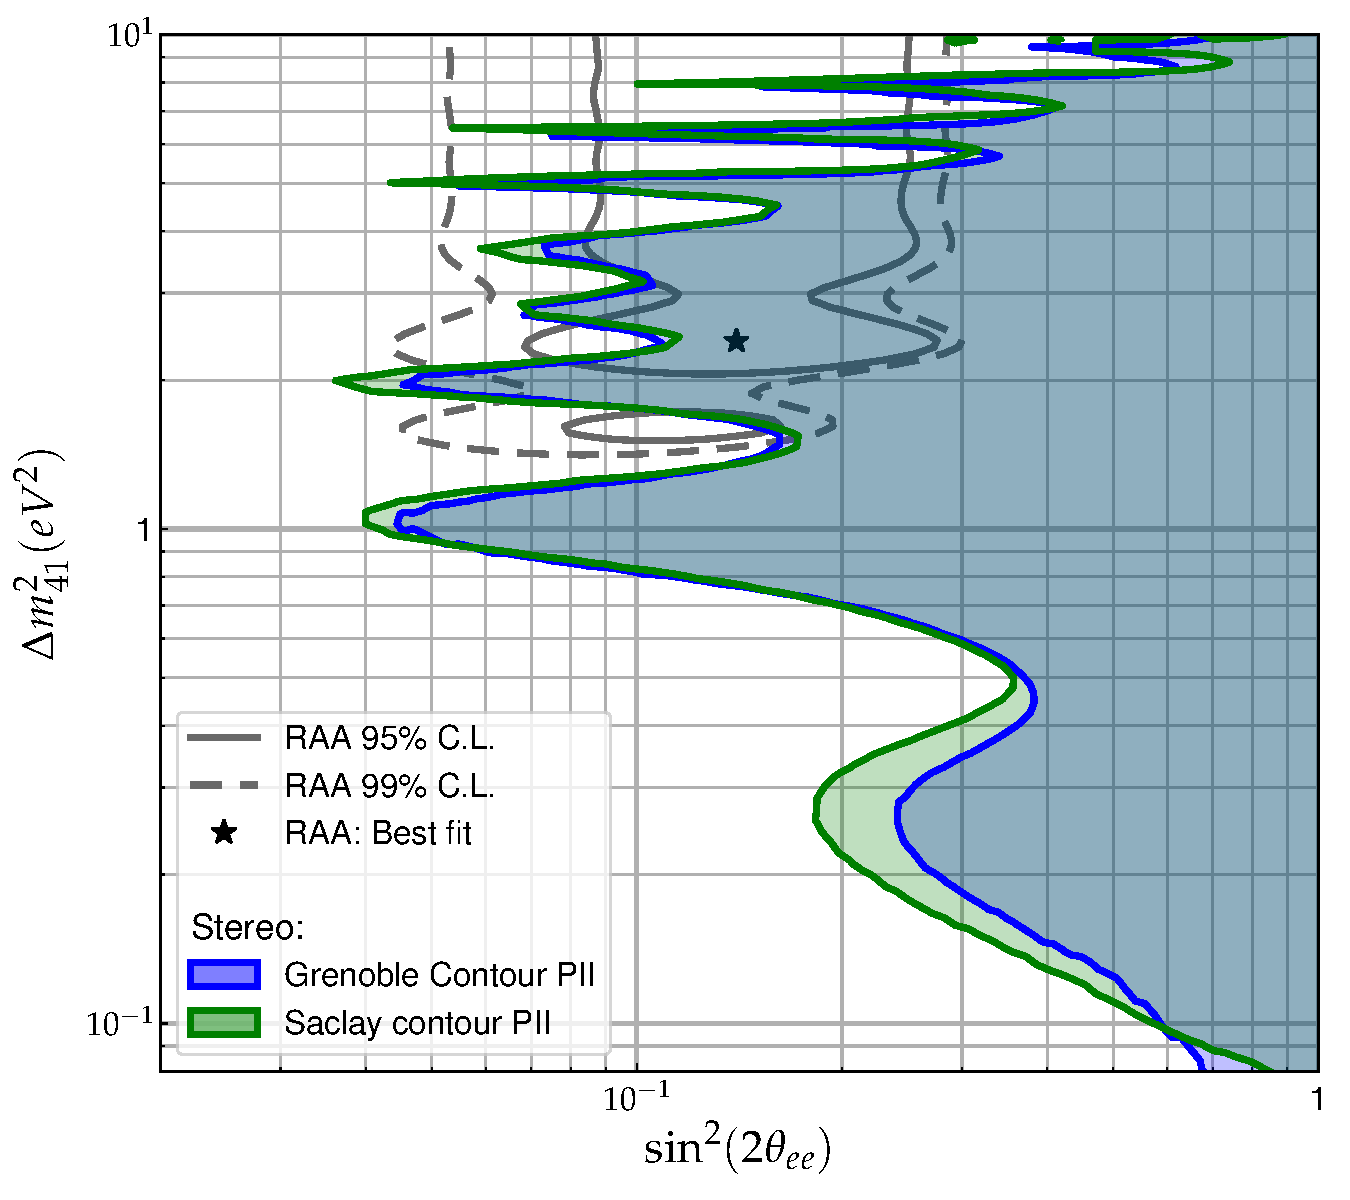
\includegraphics[width=0.75\linewidth]{images/Exclusion_Contour_Map_SvsG_PII.pdf}
  \caption[Comparaison des contours d'exclusion obtenus par la méthode de Saclay et de Grenoble]{Comparaison des contours d'exclusion obtenus par la méthode de Saclay et de Grenoble. Les deux zones colorées représentent le sous-espace des paramètres du neutrino stérile ($\Delta m_{14}^2, \textrm{sin}^2\left(2\theta_{14}\right)$) qui sont rejetés à au moins 90\% de niveau de confiance.}
  \label{fig:Exclusion_Contour_Map_SvsG_PII.pdf}
\end{figure}

\begin{figure}[h!]
  \centering
  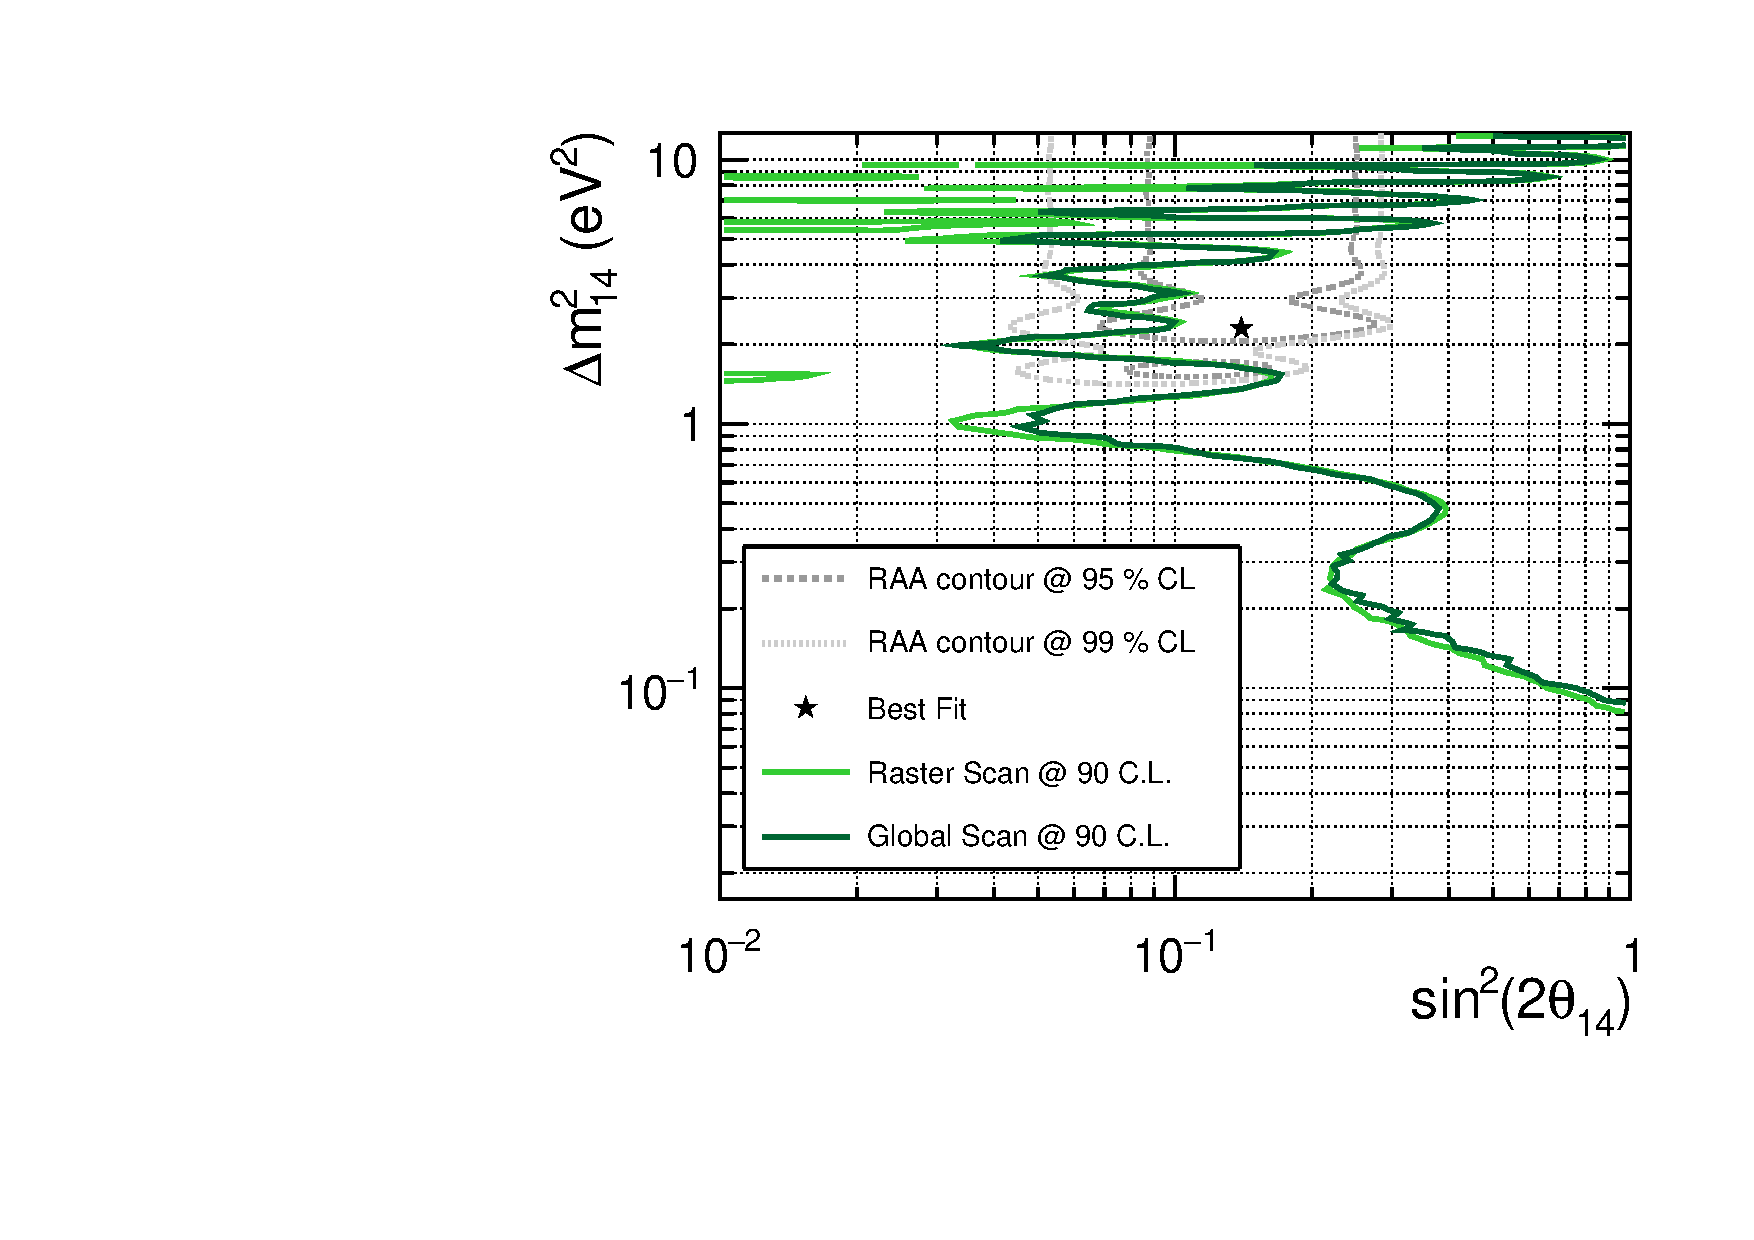
\includegraphics[width=0.75\linewidth]{images/contours_global_vs_raster_DATA.pdf}
  \caption[Comparaison des contours d'exclusion obtenus par \textit{raster-scan} et \textit{global-fit}]{Comparaison des contours d'exclusion obtenus par \textit{raster-scan} et \textit{global-fit}. Les lignes désignent le sous-espace des paramètres du neutrino stérile ($\Delta m_{14}^2, \textrm{sin}^2\left(2\theta_{14}\right)$) qui sont rejetés à au moins 90\% de niveau de confiance.}
  \label{fig:contours_global_vs_raster_DATA.pdf}
\end{figure}

\clearpage

%\begin{table}[h!]
%  \begin{center}
%    \begin{tabular}{|c|c|c|c|}
%    \hline
%      Source & $\Delta m_{14}^2 (\textrm{eV}^2)$  & $\textrm{sin}^2\left(2\theta_{14}\right)$ & Réjection de \textsc{Stereo} (C.L.) \\
%      \hline
%      \hline
%      Mention et al. (2011) \cite{Mention:2011rk} & 2.3 & 14 \% & $99.7 \% (\sim 3\sigma)$ \\
%      \hline
%      NEOS + DANSS \cite{Dentler:2018sju} & 1.3 & 4 \% & $51 \% (\sim 0.7\sigma)$ \\
%      \hline
%      Neutrino-4 \cite{Serebrov:2018vdw} & 7.3 & 44 \% & $88 \% (\sim 1.6\sigma)$ \\
%      \hline
%    \end{tabular}
%  \end{center}
%  \caption[Collection de valeurs de réjection pour quelques régions pointées par la communauté]{Collection de valeurs de réjection pour quelques régions pointées par la communauté.}
%    \label{tab:rejection_results_phase2}
%\end{table}

}

Les contours d'exclusion à 90 \% de niveau de confiance obtenu par les deux analyses complémentaires (Saclay et Grenoble) sont superposés sur la figure \ref{fig:Exclusion_Contour_Map_SvsG_PII.pdf}. Dans les deux méthodes, l'inférence statistique est établie par la génération de pseudo-expériences pour chaque point de la grille ($\Delta m_{14}^2, \textrm{sin}^2\left(2\theta_{14}\right)$). Les distributions de $\Delta\chi^2 = \chi^2_{H_x} - \chi^2_\textrm{best-fit}$ sont obtenus par \textit{raster-scan}, c'est-à-dire en cherchant le \textit{best fit} de chaque pseudo-expérience à $\Delta m_{14}$ fixé. Les valeurs de $\Delta\chi^2_{H_x}$ calculées avec données sont ensuite reportées sur l'espace des phases ($\Delta m_{14}^2, \textrm{sin}^2\left(2\theta_{14}\right)$), et la \textit{p-value} est déduite en comparant chaque $\Delta\chi^2_{H_x}$ avec sa distribution associée. Les zones colorées sur la figure \ref{fig:Exclusion_Contour_Map_SvsG_PII.pdf} désignent l'ensemble des paramètres qui ont une \textit{p-value} inférieure ou égale à 10 \% ($\textrm{exclusion C.L.} = 1 - \textit{p-value}$). Ces hypothèses sont dites \og rejetées à plus de 90 \% de niveau de confiance \fg{}.\\

% On pourrait être surpris de constater le comportement ondulatoire des contours d'exclusion pourtant non présents dans les contours de sensibilité\footnote{C'est en fait une question qui m'a été posé à plusieurs reprises lors de séminaires donnés en public. Habituellement les analyses d'oscillation incorporent les informations sur la normalisation de la simulation, c'est pour cette raison que les vagues, notamment à haut $\Delta m_{14}^2$, sont moins visibles.}. Pour expliquer ce phénomène, il faut rappeler que les données mesurées ne sont qu'une réalisation statistique d'un modèle (que l'on cherche) et donc présentent des fluctuations. Certains motifs d'oscillation en $\Delta m_{14}^2$ peuvent imiter l'allure des fluctuations statistiques. La valeur du $\chi^2$ est réduite et le pouvoir de réjection est amoindri dans la tranche en $\Delta m_{14}^2$. Ce phénomène provoque des \og creux \fg{} de sensibilité présents sur la figure \ref{fig:Exclusion_Contour_Map_SvsG_PII.pdf}. \\

Les deux méthodes (Saclay et Grenoble) montrent des zones d'exclusion très similaires. La position des pics de sensibilité sont les mêmes en $\Delta m_{14}^2$ et leurs amplitudes sont très proches dans la zone du \textit{best fit} de la RAA (représenté par une étoile). On remarque cependant que l'amplitude est plus importante avec la méthode qui exploite la matrice de covariance pour déterminer le $\chi^2$. Les raisons derrière cette différence n'ont pas encore été identifiées. Il est possible que cette différence provienne de la précision numérique avec laquelle les matrices de covariances sont inversées. Un premier indice en vertu de cette hypothèse est la nature variable de la différence de couverture en fonction de la fréquence d'oscillation $\Delta m_{14}^2$ : sur les pics de sensibilité de la méthode des matrices de covariance sur-couvre légèrement la zone de réjection tandis que dans les creux elle la sous-couvre. Cela signifie que le pouvoir de réjection de \textsc{Stereo} est légèrement surestimé par rapport à la méthode de Grenoble. Il serait intéressant d'estimer la précision numérique avec laquelle l'inversion est effectuée.\\

Les données phase 2 de l'expérience \textsc{Stereo} ont pu à elles seules exclure une bonne partie de la zone suspectée par la RAA. En particulier le best fit pointé par Mention \textit{et al.} \cite{Mention:2011rk} est rejeté à $99,7 \% (\sim 3\sigma)$.\\

% est Le Tableau \ref{tab:rejection_results_phase2} rassemble quelques valeurs pointées par la communauté.\\

Les contours de réjection ont aussi été générés selon la méthode du \textit{global-scan}. La figure \ref{fig:contours_global_vs_raster_DATA.pdf} montre la comparaison des résultats avec le \textit{raster-scan}. Les zones d'exclusion présentes à gauche du plan, qui ont été ignorées dans la figure \ref{fig:Exclusion_Contour_Map_SvsG_PII.pdf}, disparaissent en \textit{global-scan}. Du reste, les contours se superposent avec une précision satisfaisante.\\

%Il est possible que cette différence provienne de la borne inférieure de l'espace des phases en $\textrm{sin}^2\left(2\theta_{14}\right)$. La méthode de Saclay commence l'échelle à $\textrm{sin}^2\left(2\theta_{14}\right) = 10^{-1.7}$ alors que celle de Grenoble $\textrm{sin}^2\left(2\theta_{14}\right) = 10^{-2}$. Puisqu'en \textit{raster-scan} $\Delta\chi^2$ est calculé en cherchant la valeur de $\textrm{sin}^2\left(2\theta_{14}\right)$ qui minimise le $\chi^2$ pour une certaine pseudo-expérience, le fait de ne pas considérer les valeurs entre $10^{-2}$ et $10^{-1.7}$ peut légèrement affecter les distribution de $\Delta\chi^2$.\\
% NON ! cet effet décalerait mon contour vers la droite car j'aurais toujours un chi2

% TODO : ++PRECISION pourquoi les contours sont légèrement diff ? CHECK ?


% TODO : ++PRECISION global scan ?

\bigbreak


\subsection{Fusion des résultats en phase 1 et phase 2}
\label{sec:merge_phases_results}

\afterpage{

\begin{figure}[h!]
  \centering
  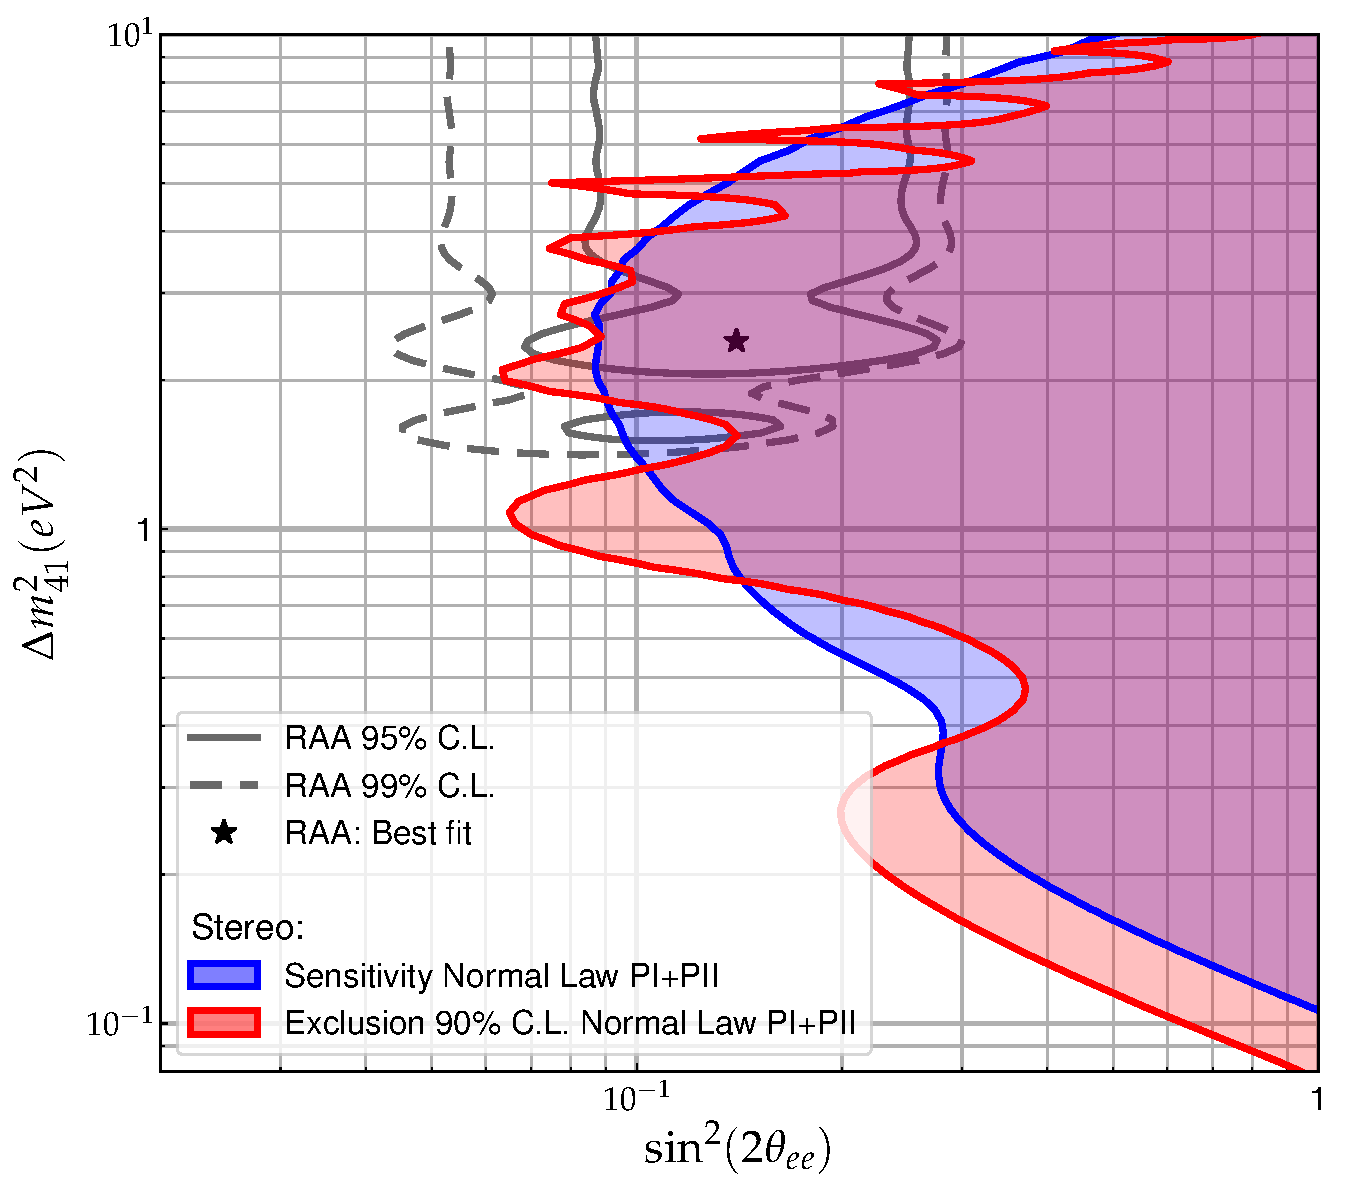
\includegraphics[width=0.75\linewidth]{images/Exclusion+Sensitivity_Contours_Map_NormalLaw_correctbinning_PI+PII_official.pdf}
  \caption[Combinaison des mesures en phase 1 et phase 2]{Combinaison des mesures en phase 1 et phase 2. Les deux phases ont été considérées comme indépendantes pour générer ces contours. L'inférence statistique est établie par \textit{raster-scan} à l'aide des lois normales de $\chi^2$. Le contour de sensibilité est tracé en bleu et la zone rejetée par les spectres mesurés en phase 1 et 2 est en rouge. Le \textit{best fit} de l'anomalie réacteur est rejeté à 99.8 \% C.L..}\label{fig:Exclusion+Sensitivity_Contours_Map_NormalLaw_correctbinning_PI+PII_official.pdf}
\end{figure}

}

Puisqu'il a été montré dans la section \ref{sec:sensitivity_phase_2_example} que les $\Delta\chi^2$ en \textit{raster-scan} suivent des lois normales à 1 degré de liberté avec une précision satisfaisante, il est possible de combiner les résultats en phase 1 et phase 2. Les opérations de maintenance menées entre les deux phases permettent de considérer les mesures indépendantes. L'expression due $\chi^2$ qui fusionne les deux périodes s'écrit simplement :

\begin{equation}
    \chi^2_{I + II} = \chi^2_{I} + \chi^2_{II},
\end{equation}

\bigbreak

où $\chi^2_{I}$ fait intervenir les données, la simulation ainsi que les erreurs de la phase 1 et $\chi^2_{II}$ pour la phase II. Pour l'évaluation du $\Delta\chi^2$, la position du \textit{best fit} est obtenue en recherchant le couple de paramètres ($\Delta m_{14}^2, \textrm{sin}^2\left(2\theta_{14}\right)$) qui minimise $\chi^2_{I + II}$, c'est-à-dire la somme des deux $\chi^2$ (et non le minimum de chaque $\chi^2$). Le degré de confiance de réjection est établi avec la loi normale à 1 degré de liberté:

\begin{equation}
    C.L.\left(\Delta\chi^2_\textrm{Data}\right) = \int_0^{\Delta\chi^2_\textrm{Data}} d\Delta\chi^2 \frac{\left( \Delta\chi^2 \right)^{-1/2} e^{-\Delta\chi^2/2}}{2^{1/2} \Gamma\left(\frac{1}{2}\right)}.
\end{equation}

\bigbreak

Les contours de sensibilité et de réjection à 90\% de niveau de confiance sont présentés sur la figure \ref{fig:Exclusion+Sensitivity_Contours_Map_NormalLaw_correctbinning_PI+PII_official.pdf}. Des études sont en cours pour les générer à l'aide des véritables PDFs du $\Delta\chi^2$ combiné.

\bigbreak

\section{Perspectives d'analyses de \textsc{Stereo}}

Les études des distorsions relatives des spectres positrons mesurés dans chaque cellule ont exclu une bonne partie de l'espace des phases des paramètres d'oscillation vers un neutrino stérile. En parallèle de la poursuite de la prise de données pour améliorer la précision statistique de l'expérience, les analyses menées dans \textsc{Stereo} se tournent aujourd'hui vers des mesures \og absolues \fg{}, c'est-à-dire des mesures qui font référence à des prédictions extérieures.\\

Cette section est consacrée à ces perspectives, en cours d'étude pendant la rédaction de cette thèse. Dans un premier temps, l'estimation du flux d'antineutrinos émis par le réacteur de l'ILL est brièvement discutée, suivie d'un point concernant la forme du spectre antineutrino pur $\ce{^{235}U}$. Enfin, le formalisme permettant de contraindre au mieux l'échelle en énergie est développé.

\bigbreak

\subsection{Test de l'anomalie réacteur}

Tester l'anomalie réacteur consiste à comparer le taux de neutrinos mesuré par rapport à une prédiction $\phi_\nu^\textrm{det}$. Sa forme définitive a été justifiée dans la Section \ref{sec:control_eff_det} :

\begin{equation}
    \phi_\nu^{\textrm{det}} = \phi_\nu^{\textrm{em}} \times \tau_\nu \times \varepsilon_d^{\textrm{tot}},
\end{equation}

\bigbreak

où $\tau_\nu$ est l'acceptance géométrique, $\varepsilon_d^{\textrm{tot}}$ l'efficacité de détection due aux coupures de sélection imposées dans l'analyse, et $\phi_\nu^{\textrm{em}}$ le taux de neutrinos émis par le réacteur. Le taux $\phi_\nu^{\textrm{em}}$ peut être obtenu de la façon suivante :

\begin{equation}
    \phi_\nu^\textrm{em} = N_{\nu / \textrm{fission}} \times N_{\textrm{fissions} / \textrm{jour}} = \frac{\left<P_{th}\right>}{\left<E_{th}^{\textrm{fission}} (\ce{^{235}U})\right>} N_{\nu_e / \textrm{fission}}(\ce{^{235}U}),
\end{equation}

\bigbreak

avec $\left<P_{th}\right>$ est la puissance thermique mesurée en temps réel lorsque le réacteur est en fonctionnement, $\left<E_{th}^{\textrm{fission}} (\ce{^{235}U})\right>$ désigne l'énergie libérée par fission et $N_{\nu_e / \textrm{fission}}(\ce{^{235}U})$ est le nombre d'antineutrinos émis par fission.\\

Le nombre de neutrinos émis par fission est calculé en intégrant le spectre de P. Huber \cite{Huber:2011wv}, corrigé des effets à basse énergie présentés à la Section \ref{sec:nu_emission} :

\begin{equation}
    N_{\nu / \textrm{fission}} = \int_{\SI{2}{MeV}}^{\SI{8}{MeV}} S^{H}_\textrm{corr} (E_\nu) dE_\nu .
\end{equation}

\bigbreak

Les bornes de l'intégrale sont déterminées par la plage considérée lors de la simulation des neutrinos. L'erreur associée à $N_{\nu / \textrm{fission}}$ est estimée à l'aide de l'incertitude théorique sur la section efficace de fission de l'$\ce{^{235}U}$ \cite{Gariazzo:2017fdh} : $\delta \sigma_{U5} / \sigma_{U5} = 2,44 \%$. La composante dominante de cette incertitude provient des spectres électron liés à la décroissance de l'$\ce{^{235}U}$ mesurés dans les années 80 à l'ILL par Schreckenbach. Celle-ci compte pour environ $2\%$. En principe, la procédure de conversion vers un spectre antineutrino ne devrait ajouter aucune erreur sur la norme, car celle-ci est totalement contrainte par les mesures électron. Néanmoins les spectres électrons n'ont été mesurés qu'à partir de $\SI{2}{MeV}$ \cite{Schreckenbach:1985ep} et le seuil de la réaction IBD ne permet pas de s'affranchir des erreurs sur la forme du spectre antineutrino \cite{Huber:2011wv}, alors  une contribution supplémentaire au bilan d'erreur de $\sigma_{U5}$ est ajoutée.\\

Le nombre de fissions par unité de temps est échantillonné à l'aide de la puissante thermique et de l'énergie libérée par fission. Cette dernière est donnée par les calculs de Ma \textit{et al.} \cite{PhysRevC.88.014605} : $\left<E_{th}^{\textrm{fission}}\right> = (202,36 \pm 0,26) \SI{}{MeV}$ pour l'Uranium 235. La puissance thermique est mesurée chaque minute à l'aide du bilan enthalpique du dispositif de refroidissement du réacteur. La procédure de mesure et son incertitude associée ont été étudiées en détail par la collaboration \textsc{Stereo} \cite{docdb342}. La puissance totale évacuée du c\oe ur peut être décomposée en quatre composantes :

\begin{equation}
    P_{th} = \sum_i P_i = P_\textrm{coeur} (\sim 96,0 \%) + P_\textrm{BP} (\sim 1,6 \%) + P_\textrm{DRG} (\sim 1,0 \%) + P_\textrm{piscine} (\sim 1,4 \%),
\end{equation}

\bigbreak

où $P_\textrm{coeur}$ est la puissance dissipée par le circuit d'eau lourde qui passe directement dans le c\oe ur, $P_\textrm{BP}$ celle du circuit au niveau de la barre de pilotage, $P_\textrm{DRG}$ la puissance évacuée par le circuit de Détection de Rupture de Gaine et enfin $P_\textrm{piscine}$ la puissance évacuée par la piscine d'$\ce{H_2O}$. Les puissances sont mesurées à partir du changement de température $\Delta T (\SI{}{^\circ C})$ qui a lieu entre l'entrée (en amont du c\oe ur) et la sortie (en aval du c\oe ur) de chaque circuit. À l'aide la capacité calorifique du matériau caloporteur $C^p (\SI{}{Jg ^\circ C^{-1}})$, la masse volumique $\rho (10^3 \SI{}{kg/m^3})$, le débit $q (\SI{}{m^3/h})$, la relation suivante est établie :

\begin{equation}
    P_i = C_i^p \times \rho_i \times q_i \times \Delta T_i
\end{equation}

\bigbreak

Les quantités $C_i^p$ et $\rho_i$ sont disponibles dans les tables de thermodynamique, tandis que les valeurs $q_i$ et $\Delta T_i$ sont mesurées par des sondes. Le débit d'eau $q_i$ est obtenu grâce à un diaphragme placé dans la tuyauterie qui induit une chute de pression en sortie de ce dernier : $q_i = \alpha \sqrt{P_\textrm{entrée} - P_\textrm{sortie}}$ où $\alpha$ est une constante de calibration. La détermination de alpha est la source dominante d'incertitude. Avant la mise en service de l'ILL le diaphragme a été placé dans une maquette à échelle 1:1 du circuit \og c\oe ur \fg{} permettant d'atteindre une incertitude relative de 0.9\% sur ce coefficient. Une telle précision est inhabituelle pour un réacteur de recherche et procure à STEREO un fort potentiel pour tester la RAA dans le cas d'un flux provenant purement des fissions d'$\ce{^{235}U}$. L'incertitude finale sur $q_\textrm{coeur}$ (la composante \og c\oe ur \fg{} est largement dominante face aux autres) est de : $\delta q_\textrm{coeur} = 1,03 \%$. L'erreur sur la différence de température $\Delta T_i$ est donnée à l'aide de la dispersion des valeurs données par les sondes redondantes. Enfin, les incertitudes sur les valeurs tabulées ($C_i^p$ et $\rho_i$) s'élèvent à hauteur de $0,1 \%$. L'erreur totale sur la puissante thermique est en définitive :

\begin{equation}
    \frac{\delta P_{th}}{P_{th}} = 1,4 \% .
\end{equation}

\bigbreak

Les deux autres quantités intervenant dans $\phi^\textrm{det}_\nu$ sont aussi porteurs d'incertitudes. L'acceptance géométrique $\tau_\nu$ est affectée à la fois par l'erreur sur l'angle solide, ainsi que le nombre de protons cibles. La résultante est :

\begin{equation}
    \frac{\delta \tau_\nu}{\tau_\nu} = 1,12 \% .
\end{equation}

\bigbreak

L'efficacité de détection totale $\varepsilon^\textrm{tot}_d$ est basée sur la simulation. L'incertitude $\delta \varepsilon^\textrm{tot}_d$ provient des désaccords de réponse entre le MC et les véritables données. Ces derniers ont été estimés à partir des analyses sur l'efficacité des coupures topologiques, les effets des biais sur l'échelle en énergie et l'efficacité de détection des neutrons. À cela s'ajoute les disparités des efficacités $\varepsilon^\textrm{tot}_d$ obtenues par deux analyses indépendantes. Cette dernière composante est en cours d'investigation. Finalement :

\begin{equation}
    \frac{\delta \varepsilon^\textrm{tot}_d}{\varepsilon^\textrm{tot}_d} = 1.72 \%.
\end{equation}

\bigbreak

\afterpage{

\begin{table}[h!]
  \begin{center}
    \begin{tabular}{|c|c|c|}
    \hline
      Composante & Incertitude relative (\%) & Source\\
      \hline
      \hline
      $N_{\nu / \textrm{fission}}$ & $2,44$ & $\delta \sigma_{U5}$ \\
      \hline
      Total Théorique & 2,44 & \\
      \hline
      \hline
      $N_{\textrm{fission} / \textrm{jour}}$ & 1,50 & $\delta P_{th}$ et $\delta \left<E_{th}^{\textrm{fission}}\right>$\\
      \hline
      \multirow{2}{*}{$\tau_\nu$} & \multirow{2}{*}{1,12} & $\delta \Omega$ (angle solide)\\
      & & + $\delta N_p$ (nombre de protons cibles)\\
      \hline
      \multirow{4}{*}{$\varepsilon^\textrm{tot}_d$} & \multirow{4}{*}{1,72} & Coupures topologiques \\
      & & + Echelle en énergie \\
      & & + Efficacité neutrino \\
      & & + Validation croisée des outils d'analyse\\
      \hline
      Total Experimental & 2,54 & \\
      \hline
    \end{tabular}
  \end{center}
  \caption[Liste préliminaire des erreurs appliquées sur la normalisation absolue du flux de neutrinos]{Liste préliminaire des erreurs appliquées sur la normalisation absolue du flux de neutrinos.}
    \label{tab:phi_det_bilan_erreur}
\end{table}

\begin{figure}[h!]
  \centering
  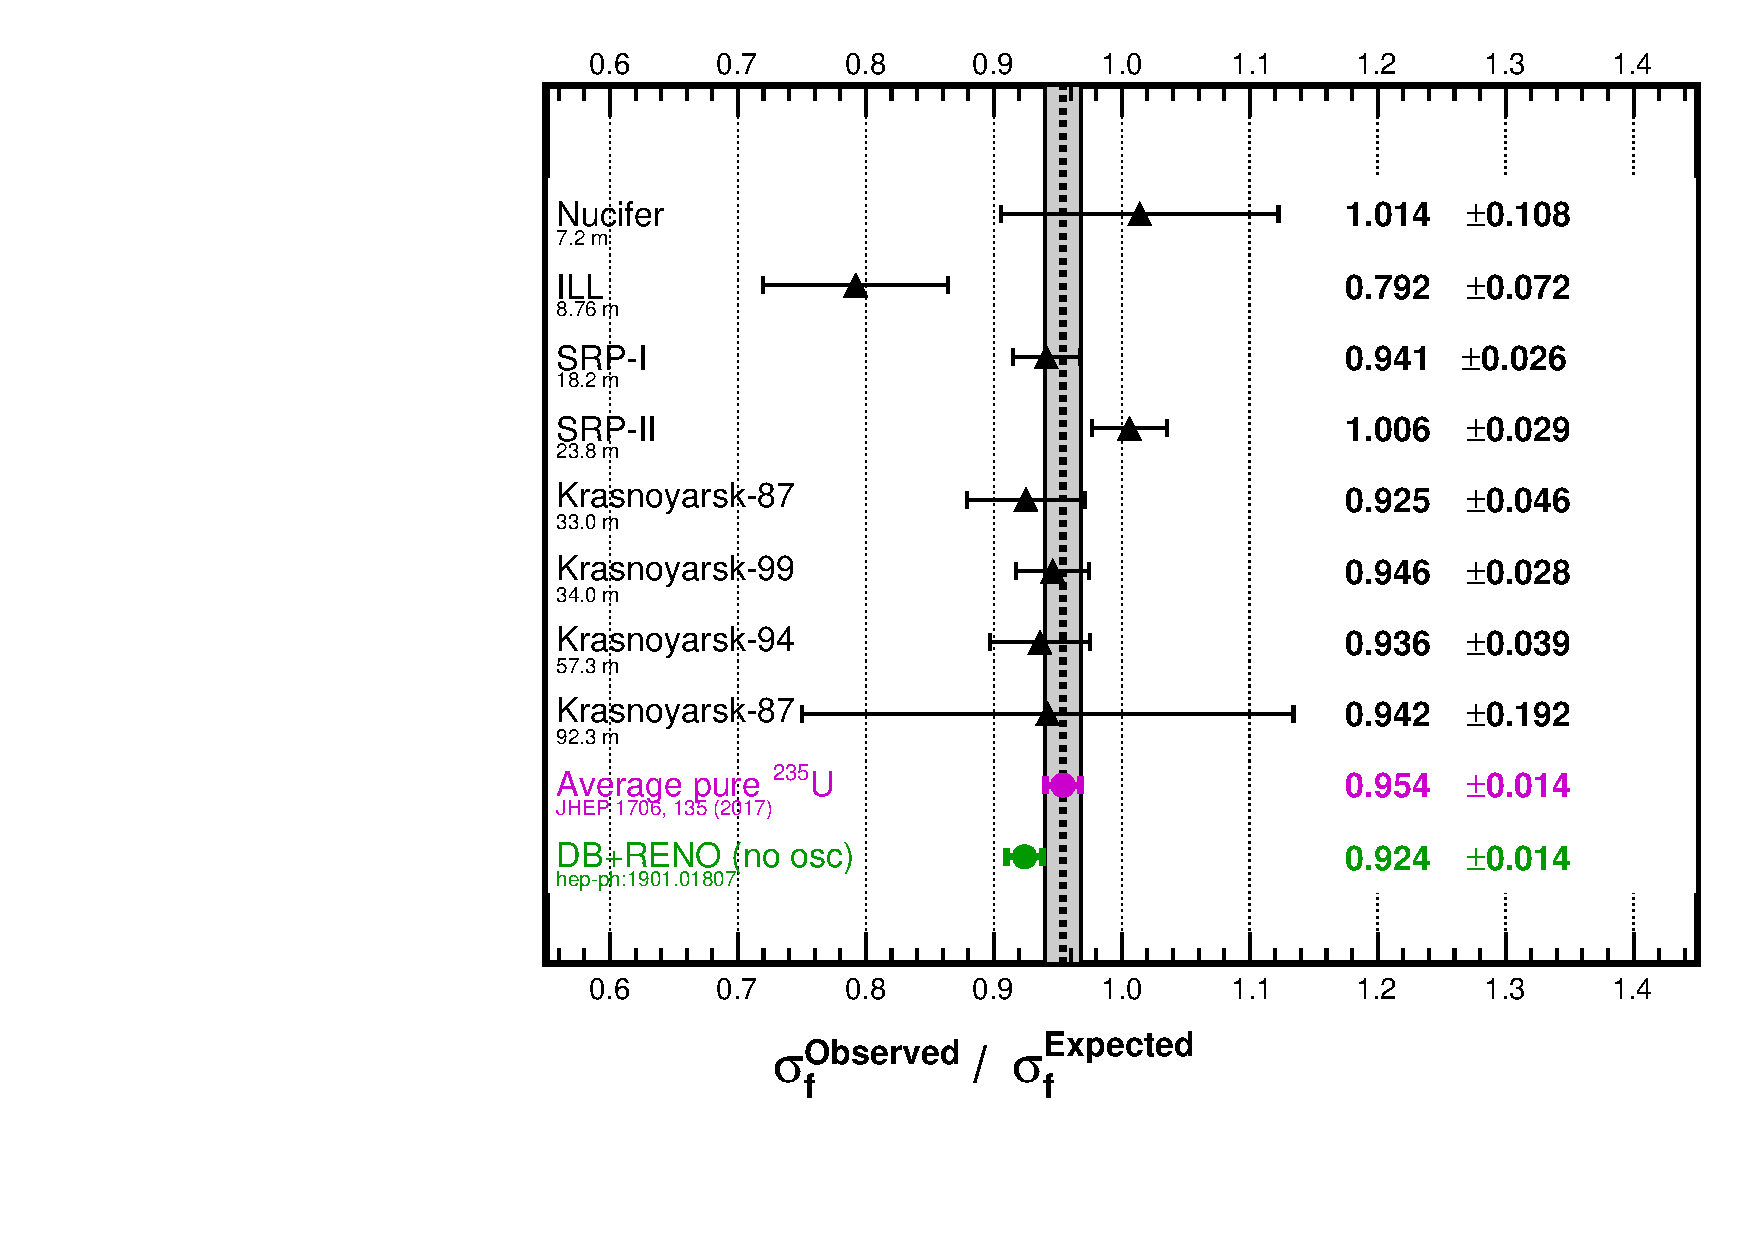
\includegraphics[width=0.8\linewidth]{images/RAA_NO_STEREO.pdf}
  \caption[Mesures de l'anomalie réacteur avec des neutrinos issus de l'$\ce{^{235}U}$]{Mesures de l'anomalie réacteur avec des neutrinos issus de l'$\ce{^{235}U}$. Les points noirs désignent les expériences ayant été conduites devant des réacteurs hautement enrichis en $\ce{^{235}U}$. La combinaison de ces résultats est représenté par le point pourpre. Cette valeur semble être en légère tension avec les résultats obtenus par décorrélation des principaux isotopes fissibles contribuant aux flux d'antineutrinos mesurés par Daya Bay et RENO (vert). \textsc{Stereo} est sur le point d'apporter sa pierre à l'édifice en fournissant une mesure supplémentaire dans la lignée des expériences pur $\ce{^{235}U}$. Les courantes estimations de l'incertitude totale placent \textsc{Stereo} comme la plus précise du marché.}\label{fig:RAA_NO_STEREO.pdf}
\end{figure}

\clearpage

}

Le bilan d'erreur est présenté sur le Tableau \ref{tab:phi_det_bilan_erreur}. Pour conclure, le calcul de l'incertitude sur $\phi_\nu^{\textrm{det}}$ est effectué avec la somme quadratique des incertitudes de chaque composante :

\begin{equation}
    \frac{\delta \phi_\nu^{\textrm{det}}}{\phi_\nu^{\textrm{det}}} = \sqrt{ \left(\frac{\delta \sigma_{U5}}{\sigma_{U5}}\right)^2 + \left(\frac{\delta P_{th}}{P_{th}}\right)^2 + \left(\frac{\delta \tau_\nu}{\tau_\nu}\right)^2 + \left(\frac{\delta \varepsilon^\textrm{tot}_n}{\varepsilon^\textrm{tot}_n}\right)^2 } = \sqrt{2,44^2_\textrm{th} + 2,54^2_\textrm{exp}} = 3,5 \%.
\end{equation}

\bigbreak

Bien que l'incertitude théorique soit commune à toutes les expériences, la composante d'erreur expérimentale place \textsc{Stereo} parmi les meilleures du marché pour mesurer le flux d'antineutrinos issus de la fission de l'$\ce{^{235}U}$. Les mesures publiées du flux de neutrinos associé à la fission de l'$\ce{^{235}U}$ sont illustrées sur la figure \ref{fig:RAA_NO_STEREO.pdf}. La moyenne des mesures effectuées auprès des réacteurs à combustible très enrichi en $\ce{^{235}U}$ montre un déficit de 6,4\%, très proche de la RAA globale incluant les mesures auprès des réacteurs commerciaux. Une approche complémentaire a été publiée par la collaboration Daya Bay puis par RENO. L'idée repose sur la grande statistique neutrino accumulée dans ces détecteurs et sur le fait que l'évolution du combustible des réacteurs commerciaux situés près de ces expériences est prédit avec précision par simulation à partir de l'historique des puissances. En regroupant les données par bins de fraction de fissions de $\ce{^{235}U}$ et $\ce{^{239}Pu}$ il est donc possible d'extraire les flux neutrinos de chaque composante. Cette analyse ressort un déficit de neutrinos liés à $\ce{^{235}U}$ plus important : 7,6\%.\\

\bigbreak

\subsection{Mesure du spectre d'émission neutrino de l'$\ce{^{235}U}$}

Plusieurs mesures auprès de réacteurs ont montré un désaccord en forme du spectre par rapport aux prédictions dans la région en énergie $[\SI{4.5}{MeV}; \SI{5}{MeV}]$. Pour cette raison, la communauté scientifique attend les résultats des expériences complémentaires ayant lieu près des réacteurs de recherche. La comparaison en forme du spectre global (les six cellules ensemble) avec une prédiction extérieure est une étude menée pendant la rédaction de cette thèse.\\

Pour cette analyse, l'extraction des spectres neutrino est effectuée avec un binning en énergie de $\SI{250}{keV}$. Bien que la résolution en énergie de \textsc{Stereo} soit similaire à celle de DayaBay \cite{DayaBay:2012aa}, il n'est pas possible de transcrire la position du bump sur l'échelle en énergie de DayaBay vers \textsc{Stereo}. En effet, puisque la nature de l'anomalie n'a pas été identifiée, il n'est pas exclu que celle-ci soit due à des effets de détection propre à la technologie employée.\\

% Il a donc été choisi de générer un Bump par dessus du modèle original (Huber corrigé, sans oscillation vers un neutrino stérile) qui est distribué selon une gaussienne dont les paramètres sont : $A$ l'amplitude, $\sigma$ la largeur et $\mu$ la position sur l'échelle en énergie.\\

Il est important de noter que pour mener cette étude, des incertitudes systématiques qui ne sont pas intervenues dans l'analyse relative doivent être prises en compte : les incertitudes sur la prédiction des spectres neutrinos. Celles-ci sont décomposées en deux parties : $\sigma^\textrm{spec}_b$ et $\sigma^{WM}$.  Les $\sigma^\textrm{spec}_b$ représentent l'erreur sur la prédiction du spectre neutrino pour chaque bin en énergie. Ils sont le résultat de la propagation de l'incertitude sur les spectres électron mesurés à l'ILL par Schreckenbach (\cite{Schreckenbach:1981wlm} et \cite{VonFeilitzsch:1982jw}), ainsi que celle sur la procédure de conversion vers le spectre neutrino ou encore l'erreur sur la méconnaissance des isotopes fissibles qui produisent les neutrinos. $\sigma^{WM}$ (pour \textit{Weak Magnetism}) incarne l'incertitude sur l'interaction des électrons avec le moment magnétique du noyau qui décroît \cite{Huffaker:1963zz}. Ainsi, la forme du $\chi^2$ employée pour comparer les données avec une prédiction peut s'écrire avec des paramètres de nuisance :

\begin{align}
    \chi^2 = \sum_c^\textrm{Cells} \sum_b^\textrm{Ebins} \left(\frac{D_{cb} - M_{cb}(\alpha_b^\textrm{spec}, \alpha^{NU}_c, \alpha^{EU}_c, \alpha^{NC}, \alpha^{EC}, \alpha^{WM})}{\sigma_{cb}^\textrm{stat}} \right)^2\\
    + \sum_b^\textrm{Ebins} \left( \frac{\alpha_b^\textrm{spec}}{\sigma_b^\textrm{spec}} \right)^2 + \sum_c^\textrm{Cells} \left( \frac{\alpha^{NU}_c}{\sigma^{NU}_c}\right)^2 + \sum_c^\textrm{Cells} \left( \frac{\alpha^{EU}_c}{\sigma^{EU}_c}\right)^2\\
    + \left( \frac{\alpha^{EC}}{\sigma^{EC}}\right)^2 + \left( \frac{\alpha^{NC}}{\sigma^{NC}}\right)^2 + \left( \frac{\alpha^{WM}}{\sigma^{WM}}\right)^2 ,
\end{align}

\bigbreak

où les termes $\alpha$ sont des paramètres qui servent à minimiser le $\chi^2$. Le spectre ajusté par les $\alpha$ est présenté sur la figure \ref{fig:absolute_spectrum_shape_analysis.png}. La valeur du $\chi^2$ minimisé par degré de liberté est de $31,8/21$, suggérant une p-value de 6 \%. Cependant, le désaccord semble essentiellement porté par les trois derniers bins en énergie. Le paramètre de nuisance sur l'échelle énergie a été repéré comme le seul déviant significativement de sa valeur nominale : $\alpha^{EC} \simeq 1,5 \sigma^{EC}$. Les déformations induites par l'échelle en énergie peuvent être responsables du désaccord à haute énergie. Par ailleurs, on pourrait être tenté d'affirmer que l'alignement des points entre 4 et $\SI{5}{MeV}$ signe la présence de l'épaulement. Néanmoins, ce phénomène pourrait aussi trouver son origine dans la méconnaissance de l'échelle en énergie. En effet, en paramétrisant les deux échelles en énergie telles que :

\afterpage{

\begin{figure}[h!]
  \centering
  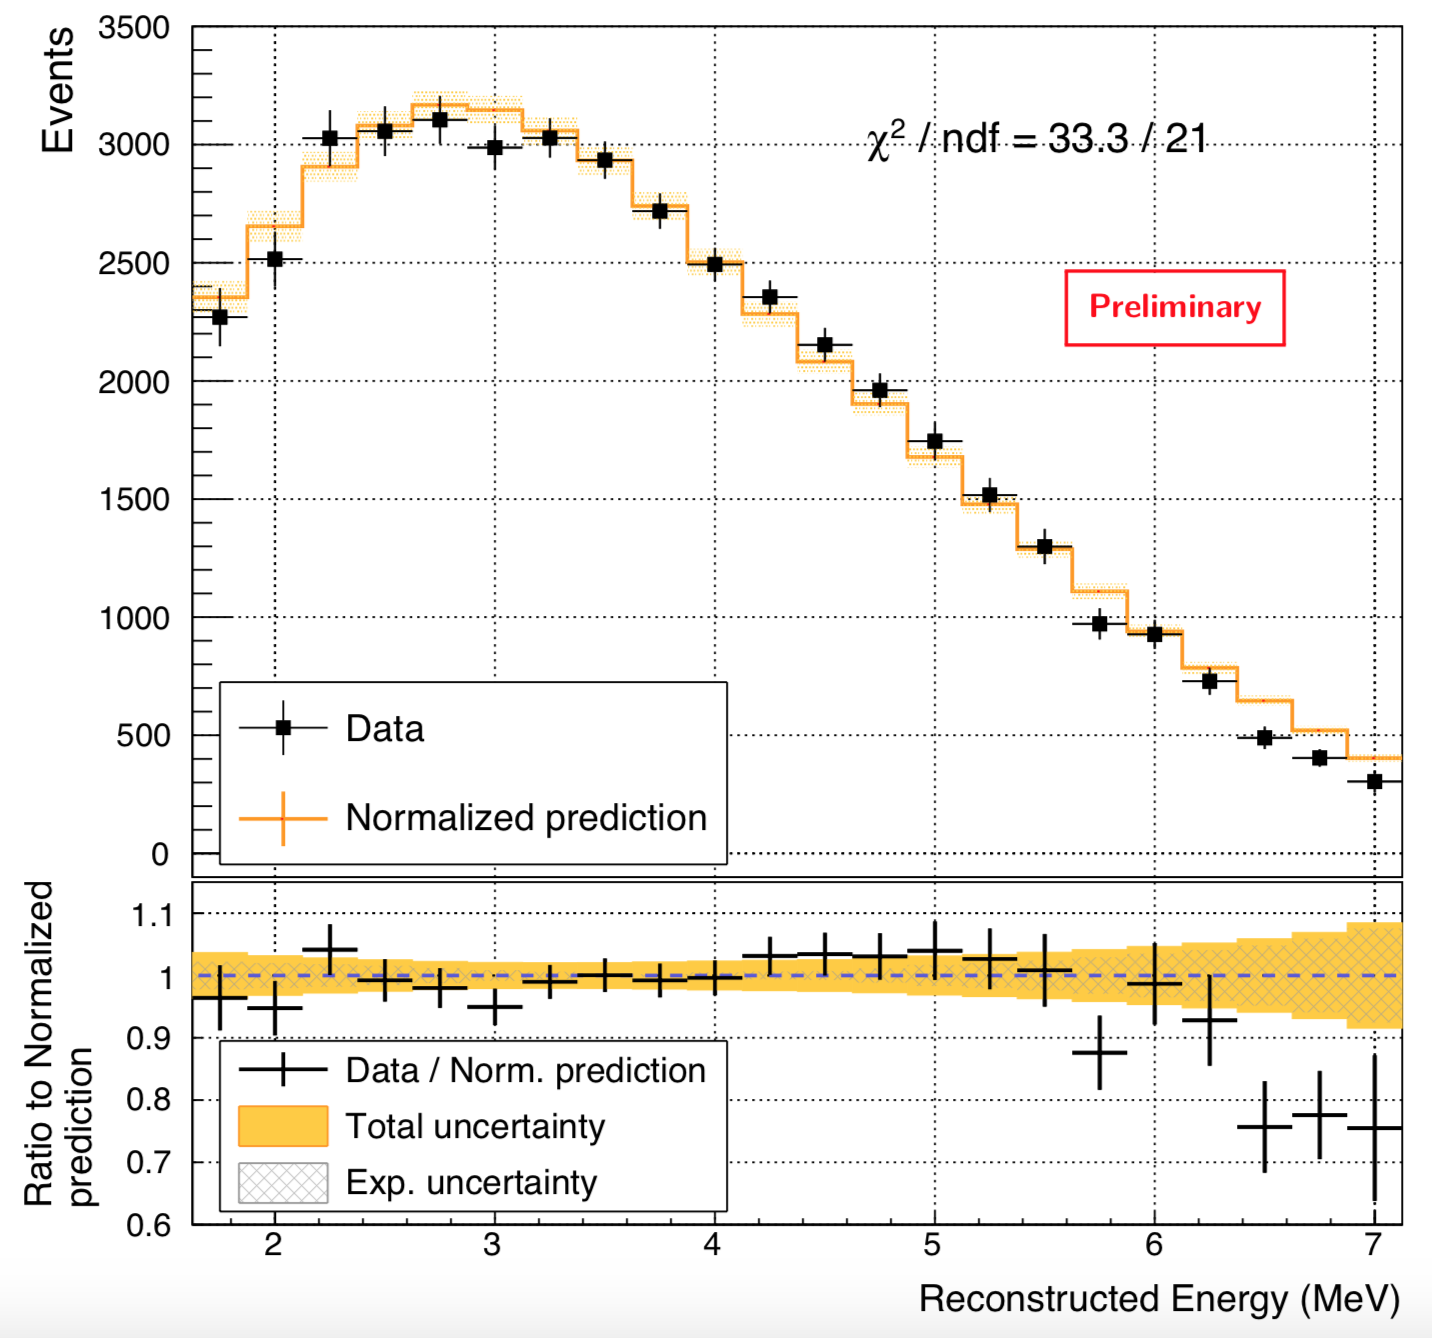
\includegraphics[width=0.75\linewidth]{images/absolute_spectrum_shape_analysis.png}
  \caption[Comparaison en forme du spectre antineutrino mesuré avec la prédiction d'Huber]{Comparaison en forme du spectre antineutrino mesuré avec la prédiction d'Huber.}\label{fig:absolute_spectrum_shape_analysis.png}
\end{figure}

}

\begin{equation}
    E_\textrm{Data} = \phi(E_\textrm{MC}) = E_{MC}\left( 1 + \delta(E_{MC}) \right),
\end{equation}

\bigbreak

il est possible d'établir le rapport de deux spectres $S_\textrm{Data}$ et $S_\textrm{MC}$ en fonction de $\delta$. Etant donné que $E_\textrm{Data} = \phi(E_\textrm{MC})$, la probabilité de mesurer une énergie dans l'intervalle $[E_\textrm{Data}, E_\textrm{Data} + dE_\textrm{Data} ]$ est la même que celle mesurée sur l'échelle de la simulation $[E_\textrm{MC}, E_\textrm{MC} + dE_\textrm{MC} ]$. Cela signifie que :

\begin{equation}
    S_\textrm{Data}(E_\textrm{Data}) dE_\textrm{Data} = S_\textrm{MC}(E_\textrm{MC}) dE_\textrm{MC}.
\end{equation}

\bigbreak

L'expression de $S_\textrm{Data}$ fait donc intervenir la dérivée de $\phi(E_\textrm{MC})$ :

\begin{equation}
\label{eq:spectrum_data_derivative_phi}
    S_\textrm{Data} = S_\textrm{MC}(E_\textrm{MC}) \times \frac{dE_\textrm{MC}}{d(\phi(E_\textrm{MC}))} = \frac{S_\textrm{MC}(E_\textrm{MC})}{\phi'(E_\textrm{MC})}.
\end{equation}

\bigbreak

En introduisant la fonction réciproque $\phi^{-1}(E_\textrm{Data}) = E_\textrm{MC}$, la dépendance en $E_\textrm{Data}$ de l'expression de $S_\textrm{Data}$ peut être restaurée :

\begin{equation}
    S_\textrm{Data}\left(E_\textrm{Data}\right) = \frac{S_\textrm{MC}\left(\phi^{-1}\left(E_\textrm{Data}\right)\right)}{\phi'\left(\phi^{-1}\left(E_\textrm{Data}\right)\right)}.
\end{equation}

\bigbreak

Au premier ordre d'un développement de Taylor en $\delta (\ll 1)$, la dépendance explicite en $E$ peut se substituer aux termes en $\phi$ :

\begin{equation}
\begin{gathered}
    \phi^{-1}(E_\textrm{Data} ) = E\times (1 - \delta(E)) + \mathcal{O}(\delta^2),\\
    \rightarrow S_\textrm{MC}\left(\phi^{-1}(E) \right) \simeq S_\textrm{MC}\left( E \left(1 - \delta\right) \right) \simeq S_\textrm{MC}(E) - E \times \delta  \times  S'_\textrm{MC}\left( E \right)    \\
    \rightarrow \frac{1}{\phi'\left(\phi^{-1}(E)\right)}  \simeq 1 - \delta\left(E\right) - E \times \delta'\left(E\right) + \mathcal{O}\left(\delta\delta', \delta\delta''\right),
\end{gathered}
\end{equation}

\bigbreak

où la contribution des termes en $\delta\delta'$ et $\delta\delta''$ sont de second ordre car $\delta(E)$ est supposé suffisamment lisse. Le rapport des spectres $S_\textrm{Data}/S_\textrm{MC}$ s'écrit finalement :

\begin{equation}
\label{eq:spectrum_non_linearities}
\begin{split}
    R^\textrm{spec}(E) = \frac{S_\textrm{Data}}{S_\textrm{MC}} & = \frac{1}{\phi'\left(\phi^{-1}\left(E\right)\right)}\frac{S_\textrm{MC}\left(\phi^{-1}\left(E\right)\right)}{S_\textrm{MC}\left(E\right)}\\
    & \simeq 1 - \delta(E) - E \left\{ \delta'(E) + \delta(E) \frac{S'_\textrm{MC}(E)}{S_\textrm{MC}(E)} \right\}
\end{split}
\end{equation}

\bigbreak

Une distorsion $\delta(E)$ sur l'échelle en énergie affecte le rapport des spectres par un terme linéaire, mais aussi via des effets locaux qui se manifestent par la dérivé du spectre $S_{MC}$ et de $\delta$. De plus ces effets locaux sont échelonnés par $E$, donc ils peuvent être dominant à haute énergie. La bosse à $\SI{5}{MeV}$ est située dans la zone où le spectre neutrino s'écroule très rapidement, une grande valeur de $S'(E)$ est donc attendue alors la moindre distorsion de l'échelle en énergie $\delta$ peut affecter fortement $R^\textrm{spec}$. Pour résumer, la formule (\ref{eq:spectrum_non_linearities}) montre qu'il est nécéssaire de contraindre l'ensemble de l'échelle en énergie avant d'interpréter les écarts entre les spectres mesurés et prédits.\\


 % Des travaux sont en cours pour contraindre l'échelle en énergie à partir des données acquises jusqu'alors.\\

%Les travaux menés par Mention \textit{et al} \cite{Mention:2017dyq} ont montré qu'il était possible d'expliquer les anomalies de forme du spectre antineutrino par une distorsion de l'échelle en énergie. Malgré 

% Ce point est brièvement discuté dans la section suivante.\\

% Les mesures fournies par DayaBay suggèrent un Bump à hauteur de 10 \% (représenté par la courbe en pointillés bleu), mais une telle déviation n'apparait pas sur les résidus des données \textsc{Stereo}.

% Pour délibérer sur la présence d'un bump ou non, l'inférence statistique est établie avec un $\Delta \chi^2$, où l'hypothèse nulle est le spectre d'Huber sans Bump ($A \doteq 0$) et le \textit{best fit} est recherché dans l'espace des paramètres de la gaussienne $A$, $\sigma$, $\mu$. Similairement aux hypothèses du neutrino stérile, les résultats pourront être présentés sous forme de contours d'exclusion.\\

\bigbreak

\subsection{Analyse approfondie sur l'échelle en énergie}

% Cette analyse a pour but de trouver la distorsion la plus probable de l'échelle en énergie ($\delta(E)$) à partir de l'ensemble des données de calibration. Ainsi, à chaque valeur de l'échelle en énergie, la distorsion locale $\delta(E)$ et son incertitude associée donnent une enveloppe dans laquelle les paramètres de nuisance $\alpha (E)$ peuvent agir dans le $\chi^2$. L'estimation par noyau est exploitée pour paramétriser $\delta(E)$ :
%
%\begin{equation}
%    \delta(E) = \sum_{k = 1}^n \omega_k \mathcal{G}_k\left(\frac{E-E_k}{h} \right),
%\end{equation}

% avec $\mathcal{G}_k$ les gaussiennes dont les paramètres sont $E_k$ et $h$, et $\omega_k$ les poids associés à chaque $\mathcal{G}_k$. Les $\omega_k$ sont les paramètres de l'ajustement du $\chi^2$ qui quantifie l'accord entre les calibrations des véritables données et la simulation. Les $E_k$ sont espacés à intervalles réguliers pour laisser $\delta(E)$ s'ajuster sur toute la gamme en énergie des neutrinos. Enfin, le paramètre $h$ gouverne la façon dont les gaussiennes se chevauchent et induisent une corrélation entre les $\omega_k$. Il a été choisi de travailler avec un $h$ comparable à l'espacement des $E_k$.\\

Une étude a été menée durant le stage de pré-thèse de Rudolph Roggly pour appliquer le formalisme développé dans \cite{Mention:2017dyq}. Cette analyse a pour but de traiter l'ensemble des contraintes offertes par les données de calibration pour cerner au mieux la forme de $\delta(E)$. Les sources de calibration donnent des contraintes ponctuelles sur l'échelle en énergie. Ces contraintes sont formalisées par le rapport d'énergie construite dans la simulation et les données :

\begin{equation}
    R^\textrm{calib}_i(E) = \frac{E^\textrm{Data}_i }{E^\textrm{MC}_i} = 1 + \delta(E).
\end{equation}

\bigbreak

Cependant, il existe très peu de sources radioactives gamma au delà de $\SI{5}{MeV}$. Pour contraindre la haute partie du spectre neutrino, il est nécéssaire de faire intervenir d'autres données. La décroissance du Bore 12 qui a été présentée dans le chapitre \ref{chap:chapitre_energie} offre un spectre électron qui s'étale jusqu'à $\SI{13.4}{MeV}$. Puisqu'il s'agit d'un spectre, l'équation (\ref{eq:spectrum_non_linearities}) donne la relation entre $\delta(E)$ et le rapport données/simulation du contenu de chaque bin. L'ensemble des contraintes sur l'échelle en énergie sont finalement rassemblées dans un vecteur :

\begin{equation}
    \overrightarrow{R} = \left(\begin{matrix}
        \overrightarrow{R}^\textrm{calib} \\
        \overrightarrow{R}^\textrm{12B}
    \end{matrix} \right).
\end{equation}

 L'ajustement de la fonction $\delta(E)$ est exécuté au moyen d'un test de $\chi^2$. En considérant une paramétrisation $\omega_k$ de la fonction $\delta(E)$, le $\chi^2$ prend la forme suivante :

\begin{equation}
    \chi^2 = \sum_i \sum_j \left( R_i - 1 - \sum_k A_{ik}\omega_k \right) V_{ij}^{-1} \left( R_j - 1 - \sum_l A_{jl}\omega_k \right) \doteq \norm{\left(R - 1\right) - A\omega}^2_{V^{-1}},
\end{equation}

\bigbreak

avec les termes en $A_{ik}$ qui représentent la façon dont est affectée la contrainte $R_i$ par le paramètre libre $\omega_k$, et $V_{ij}^{-1}$ est la matrice de covariance entre les rapport $i$ et $j$. La minimisation du $\chi^2$ à l'aide des $\omega_k$ permet de trouver le meilleur ajustement de $\delta(E)$ d'après toutes les contraintes $R_i$. La valeur ajustée $\widetilde{\delta}(E)$ ne donne cependant que la valeur la plus probable de la distorsion de l'échelle en énergie. Pour propager les résultats de cette analyse dans l'inférence sur la comparaison des spectres neutrino, les spectres simulés doivent être corrigés avec $\widetilde{\delta}(E)$ et les systématiques sur l'échelle en énergie doivent correspondre à l'incertitude sur $\widetilde{\delta}(E)$. L'enveloppe d'incertitude sur la fonction $\widetilde{\delta}(E)$ est obtenue par la matrice de covariance des $\omega_k$ :

\begin{equation}
    \sigma^2(E) = \sum_i\sum_j \frac{\partial \delta(E)}{\partial \omega_i} V(\omega_i, \omega_j) \frac{\partial \delta(E)}{\partial \omega_j}.
\end{equation}

\bigbreak

En pratique, une paramétrisation envisageable pour $\delta(E)$ est par exemple donnée par un polynôme de second ordre :

\begin{equation}
\begin{gathered}
    E_\textrm{Data} = a + b \times E_\textrm{MC} + c \times E_\textrm{MC}^2 \\
    \Rightarrow \delta(E) = \frac{a}{E_\textrm{MC}} + b - 1 + c\times E_\textrm{MC}.
\end{gathered}
\end{equation}

\bigbreak

où $a$ décrit un potentiel biais sur l'échelle en énergie, $b$ teste la précision relative de l'étalonnage entre les données et le MC, et enfin $c$ prend en compte des non linéarités résiduelles. Le modèle de distorsion par un polynôme du second ordre permet d'éviter les sur-ajustements de $\delta(E)$. De plus, il se justifie dans la mesure où $b$ reste proche de 1 et où les autres termes contribuent très peu dans la gamme d'énergie exploitée par \textsc{Stereo}.  

\bigbreak

%\afterpage{
%
%\begin{figure}[h!]
%  \centering
%  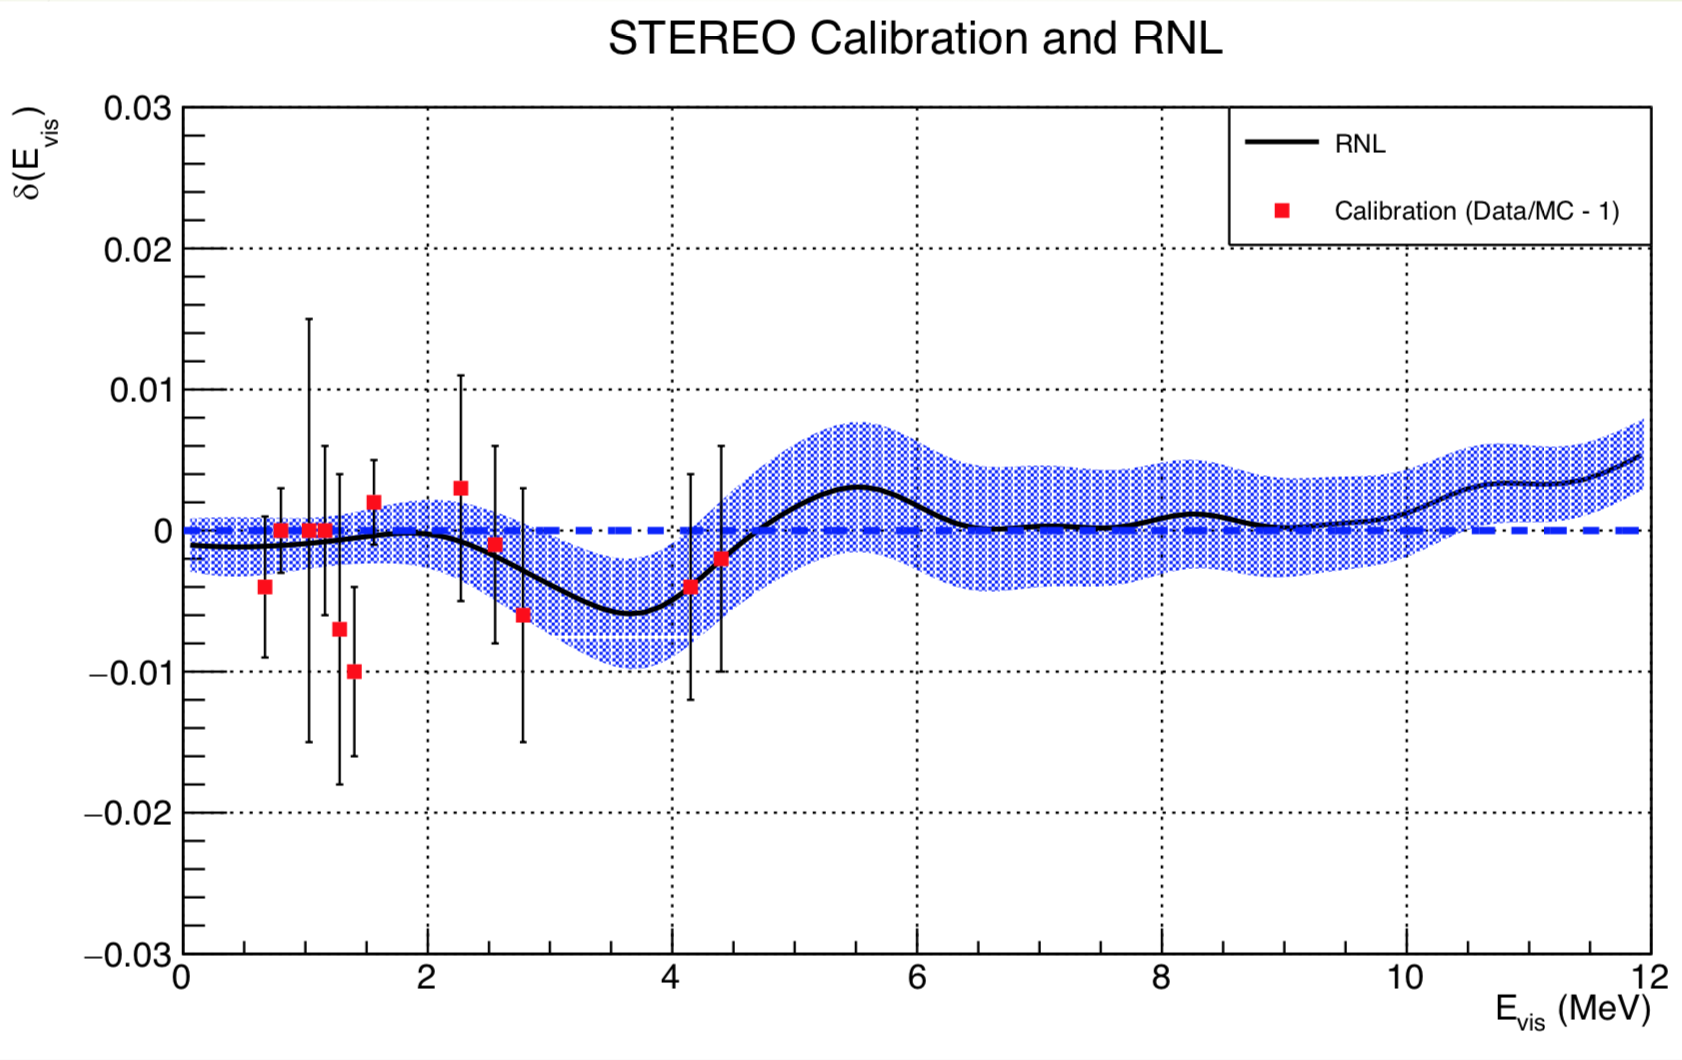
\includegraphics[width=0.95\linewidth]{images/general_E_scale_fit.png}
%  \caption[Exemple d'ajustement de la fonction exprimant les non-linéarités résiduelles de l'échelle en énergie]{Exemple d'ajustement de la fonction exprimant les non-linéarités résiduelles (RNL) de l'échelle en énergie. La RNL représente la fonction $\delta(E)$ ajustée par le $\chi^2$, et la zone bleue est l'enveloppe représentant l'incertitude locale sur $\delta(E)$. Cette fonction a été ajustée sur les données de calibration avec les sources radioactives ainsi qu'avec le spectre du Bore 12 mesuré et simulé.}
%  \label{fig:general_E_scale_fit.png}
%\end{figure}
%
%
%}

% Un exemple d'ajustement est présenté sur la figure  \ref{fig:general_E_scale_fit.png}. La fonction $\delta(E)$ ajustée avec le $\chi^2$ est appelée RNL (pour \textit{Residual Non Linearity}). Celle-ci donne la distorsion la plus probable de l'échelle en énergie qui s'applique sur le spectre neutrino. Ainsi, pour apporter un traitement plus approfondi des distorsions de l'échelle en énergie sur la comparaison des spectres positrons, les prédictions $M_{cb}$ doivent être corrigées au préalable de $\delta(E)$ ($M_{cb} = \overline{M}_{cb} + \delta(E) \eta_{cb}$) et les paramètres de nuisances sur l'échelle en énergie $\alpha^{EC}$ sont libres de varier sur une gamme définie par l'erreur de la RNL : $\sigma^2(E)$.

\bigbreak

\subsection{Vers une nouvelle référence en forme du spectre $\ce{^{235}U}$}

Ce formalisme peut aussi servir à trouver les distorsions nécessaires sur la prédiction des spectres antineutrino d'Huber pour ajuster les spectres positron mesurés et simulés :

\begin{equation}
    S_{\nu}(E) = S^{H}_{\nu}(E) + \delta(E),
\end{equation}

\bigbreak

où $S^{H}_{\nu}(E)$ est la prédiction d'Huber. Attention, cette fois $\delta(E)$ représente une distorsion de la forme du spectre antineutrino et non une déformation de l'échelle en énergie. Pour effectuer cette analyse, $\delta(E)$ peut prendre la forme d'une fonction d'estimation de densité par noyau (non-paramétrique) : 

\begin{equation}
    \delta(E) = \sum_{k = 1}^n \omega_k \mathcal{G}_k\left(\frac{E-E_k}{h} \right),
\end{equation}

avec $\mathcal{G}_k$ les gaussiennes dont les paramètres sont $E_k$ et $h$, et $\omega_k$ les poids associés à chaque $\mathcal{G}_k$. Les $E_k$ sont espacés à intervalles réguliers pour laisser $\delta(E)$ s'ajuster sur toute la gamme en énergie des neutrinos. Enfin, le paramètre $h$ gouverne la façon dont les gaussiennes se chevauchent et induisent une corrélation entre les $\omega_k$. En vue d'estimer $\hat{\delta}(E)$, la statistique $\chi^2$ suivant est utilisé :

\begin{equation}
    \chi^2 = \norm{D_{cb} - M_{cb}\left(S_\nu(E) + \delta(E)\right)}^2_{V^{-1}} + \lambda \int \delta^{''}(E) dE,
\end{equation}

\bigbreak

avec $M_{cb}(S^{H}_\nu(E) + \delta(E))$ représentant le spectre positron simulé à partir du spectre antineutrino distordu $S_{\nu}(E)$. $M_{cb}$ peut être calculé à la volée à l'aide d'une matrice de réponse qui établit la relation entre énergie des neutrinos et énergie reconstruite des positrons. Puisque $\delta(E)$ est un estimateur non paramétrique, il est nécessaire d'ajouter un terme de régularisation dont l'amplitude est donnée par $\lambda (\geq 0)$ afin d'éviter les sur-ajustements. Ici, la contrainte est donnée sur la dérivée seconde de $\delta(E)$ : cela traduit le fait que l'on souhaite obtenir une fonction $\hat{\delta}(E)$ suffisamment lisse pour ignorer les fluctuations statistiques des spectres. Lorsque $\lambda$ est faible, le terme de régularisation n'impose pas de contraintes sur $\delta(E)$, impliquant que la fonction $\delta(E)$ qui minimise le $\chi^2$ risque d'être sur-ajusté sur les données. Si maintenant $\lambda$ est grand, le terme de régularisation domine dans le $\chi^2$, forçant la minimisation à garder la dérivée seconde de $\delta$ nulle en tout point de l'échelle en énergie. Cela signifie que les déformations autorisées tendent vers $\delta(E) = a \times E + b$, où $a$ et $b$ sont des constantes.\\

La \og bonne \fg{} valeur de $\lambda$ peut être obtenue par \og \textit{Generalized Cross-Validation} \fg{} (GCV) explicitée par \cite{10.2307/1268518}. Cependant l'implémentation de cette méthode ainsi que l'étude du choix de binning en $E_k$ et la largeur des gaussiennes $h$ sont encore en cours d'étude pendant la rédaction de ce manuscrit.\\


%Puisque les $\omega_k$ ajustés (dénotés avec un chapeau $\hat{\omega}$) sont linéaires avec $(R_i - 1)$, il est possible d'écrire :
%
%\begin{equation}
%    \hat{R} - 1 = A \hat{\omega} = H(\lambda)(\hat{R} - 1),
%\end{equation}
%
%\bigbreak
%
%où $H(\lambda) = A P(\lambda)$, avec $P(\lambda)$ la matrice de passage permettant d'exprimer la covariance des $\hat{\omega}$ en fonction de la matrice de covariance dans la base des $(\hat{R} - 1)$. Ensuite, la relation suivante peut être exprimée en fonction de $H(\lambda)$ :
%
%\begin{equation}
%    R - \hat{R} = (R - 1) - (\hat{R} - 1) = (I - H(\lambda)) (R - 1)
%\end{equation}
%
%\bigbreak
%
%La GCV consiste à minimiser l'expression suivante pour trouver le $\lambda$ adéquat :
%
%\begin{equation}
%    GCV(\lambda) = \frac{\norm{R - \hat{R}}^2_{V^{-1}}}{Tr\left[I - H(\lambda)\right]^2} = \frac{\norm{(I - H(\lambda)) (R - 1)}^2_{V^{-1}}}{Tr\left[I - H(\lambda)\right]^2}.
%\end{equation}

Pour conclure, l'avantage du déploiement d'un tel formalisme est de pouvoir fusionner les résultats obtenus par plusieurs expériences. En effet, si les distorsions sont ajustées avec le même binning en $E_k$, les distorsions combinées peuvent être exprimées à partir des résultats de chaque expérience ($\hat{\omega}, V(\hat{\omega})$):

\begin{equation}
    \hat{\omega}_\textrm{combiné} = \frac{\left( V(\hat{\omega})^{-1}_\textsc{Stereo} \hat{\omega}_\textsc{Stereo} + V(\hat{\omega})^{-1}_\textsc{X} \hat{\omega}_\textsc{X} \right)}{V(\hat{\omega})^{-1}_\textsc{Stereo} + V(\hat{\omega})^{-1}_\textsc{X}},
\end{equation}

\bigbreak

où $X$ désigne une autre expérience mesurant le spectre antineutrino pur $\ce{^{235}U}$ (par exemple PROSPECT ou SoliD). Une nouvelle prédiction des spectres antineutrino associés à l'$\ce{^{235}U}$ pourra ainsi être déduite en propageant $\hat{\omega}_\textrm{combiné}$ sur $S_\nu(E)$.

\bigbreak

%\section{Comparaison des données \textsc{Stereo} avec des prédictions extérieures}
%
%\subsection{L'anomalie réacteur}
%
%\subsection{Comparaison de la forme des spectres avec une prédiction}
%
%\section{Les expériences concurrentes}
%
%\subsection{PROSPECT}
%
%\subsection{SoLi$\delta$}
%
%\subsection{Neutrino-4}

